\documentclass{dissertation}
% FIGURES
\usepackage{xr} 
\usepackage{graphicx}
\usepackage{rotating}
\usepackage{wrapfig}
% \usepackage{epstopdf}
\usepackage[font={small, it},      % small caption size
labelfont=bf,                % bold "Figure"
labelsep=period]{caption}    % separate Figure from text swith period
\usepackage[section]{placeins} % always place figures in section

% CHEMICAL FORMULAS
\usepackage[version=3]{mhchem} 	% Formula subscripts using \ce{}
\usepackage{chemformula}

% PHYSICAL UNIT FORMATTING
\usepackage[separate-uncertainty = true,
detect-all = true,
range-phrase = --,
range-units = single,
list-units = single,
multi-part-units = single]{siunitx}
\DeclareSIUnit[number-unit-product = {}]\uL{ \micro\liter}
\DeclareSIUnit[number-unit-product = {}]\fL{ \femto\liter}
\DeclareSIUnit[number-unit-product = {}]\umol{ \micro \mole}
\DeclareSIUnit[number-unit-product = {}]\mM{ \milli M}
\DeclareSIUnit[number-unit-product = {}]\uM{ \micro M}
\DeclareSIUnit[number-unit-product = {}]\nM{ \nano M}
\DeclareSIUnit[number-unit-product = {}]\pM{ \pico M}
\newcommand*\me[1]{\ensuremath{\bar{#1}\,}}

% MISC
\newcommand{\squeezeup}{\vspace{-2.5mm}}
%=============== extra: martin binfree =====================
% preamble:
\usepackage{amsmath}    % need for subequations
\usepackage{mathrsfs}   % for laplace simbol
\usepackage{verbatim}   % useful for program listings
\usepackage{color}      % use if color is used in text
\usepackage{subfigure}  % use for side-by-side figures
\usepackage{hyperref}   % use for hypertext links, including those to external documents and URLs
\raggedbottom           % don't add extra vertical space
\usepackage{dcolumn}% Align table columns on decimal point
\usepackage{bm}% bold math


\newcommand{\ve}[1]{{\mathbf{#1}}}
%%%%%%%%%%%%%%%%%%% MAIN PART %%%%%%%%%%%%%%
\begin{document}
\title[]{Fluorescence of Single Copper Proteins: Dynamic Disorder and Enhancement by a Gold Nanorod}
\author{Biswajit}{Pradhan}
%\input{title}
%\chapter*{Preface}
\addcontentsline{toc}{chapter}{Preface}
\setheader{Preface}

Preface goes here. This chapter is optional.

\begin{flushright}
{\makeatletter\itshape
    \@firstname\ \@lastname \\
    Leiden, January 2018
\makeatother}
\end{flushright}
\tableofcontents
\mainmatter
%==========Chapters================
\thumbtrue
% \chapter{Introduction}
\label{chapter:intro}
\graphicspath{{./chapters/c1_intro/figures/}}
%=========== MAIN ================
Single-molecule fluorescence was invented in the 1990s and has quickly developed into an indispensable technique in the biomedical sciences and condensed matter research. It has revolutionized the fields of molecular biology, imaging (super-resolution), or catalysis, to name a few. In this thesis, we will apply fluorescence enhancement by single gold nanorods to extend single-molecule studies to chromophores with low fluorescence quantum yields and to high concentrations of probe molecules. Following single-molecule trajectories, we will explore variations in the electron transfer rates of the metalloprotein azurin both from molecule to molecule and for the same molecule as a function of time, dynamically. Evidence for conformational substates will be discussed based on dynamic heterogeneity. In this introduction we have tried to cover the basic principles required in the rest of the thesis.  


\section{Fluorescence}
The absorption and subsequent emission of light by materials is called fluorescence.
The term fluorescence was named by \textit{George Gabriel Stokes} after he observed the transformation of ultraviolet light into visible light in the mineral fluorite.\cite{Stokes1852} Fluorescence was later observed in organic molecules, and this is the main subject of this work.
A molecule is excited to an excited electronic state after absorbing a resonant photon.
Each electronic energy level is associated with vibrational and rotational energy levels.
The excess vibrational energy gained in the excited state is quickly dissipated in the molecular surroundings on picosecond time scales and the molecule ends up in a thermalized excited state, where it remains for the excited-state lifetime. Depending on the spin of the excited state, a transition to the singlet ground state may be spin-allowed and lead to fluorescence emission with a lifetime typically of the order of \SIrange{1}{10}{\ns}. The emitted fluorescence photon has lower energy than the excitation photon. The associated frequency shift is known as Stokes's shift.
If the excited state is a triplet (spin 1), the transition is spin-forbidden and the lifetime usually lies in the ms to microsecond range. The associated emission is called  phosphorescence and is often observed at longer waves than fluorescence.
Absorption and emission processes are often represented graphically in a Jablonski diagram.\cite{RohatgiMukherjee1979k,Lakowicz1999book}

\begin{figure}
	\centering
	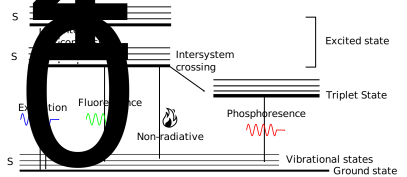
\includegraphics[width=0.8\textwidth]{jablonski}
	\caption{\textbf{Jablonski Diagram.} Simplified model of the transitions involved in fluorescence. A molecule is promoted to the excited electronic state by absorption of a photon. Non-radiative relaxation processes bring the molecule to the lowest vibrational states of the lowest excited electronic state from where it can either emit a photon or release excess electronic excitation energy as heat, making a transition to the lower-lying triplet state or singlet ground state.}
	\label{fig:jablonski}
\end{figure}

Natural materials that show fluorescence include minerals, tissue in plants and animals.
Nicotinamide adenine dinucleotide (NADH), flavins (FAD), and chlorophyll are a few examples of common biological molecules which emit significant fluorescence.\cite{blacker2014separating,siano1989nadh,genty1989the}
Alternatively, artificial fluorophores can be synthesized and used for labelling biological structures. These fluorophores present high fluorescence quantum yields and can be produced in a broad variety of colors. They include synthetic organic dyes and semiconductor nanocrystals called quantum dots.\cite{atkinson1952the,alivisatos1996semiconductor}
The greatest advantage of fluorescence is its very low background, which enables the detection of exceedingly low concentrations of fluorescent molecules, down to the single-molecule level.
This was very important for biological imaging as minute quantities of such markers keep the system under study nearly unaffected.\cite{white1987an}
Not only external fluorophores can be used for biological marking, cells can also be gene-edited to produce their own fluorophores, notably the peptide label called green fluorescent protein (GFP) and a broad variety of similar auto-fluorescent proteins.\cite{tsien1998the,chalfie1994green}
Nowadays, biological or analytical chemical experiments are virtually unthinkable without fluorescence techniques.

\section{Single-Molecule Spectroscopy}
The thought experiment by Jean Perrin to observe single fluorescent molecules was realized for the first time in 1990 at an extremely low temperature and in an advanced laboratory.\cite{orrit1990single}
The rapid development of optical microscopes, lasers, dyes and detectors soon made it possible to detect single molecules at room temperature even on a bench top.\cite{xie1998optical,weiss1999fluorescence,moerner1999illuminating}
Single-molecule spectroscopy has grown into an important research field, but is also heavily used in molecular biology, super-resolution microscopy, quantum computing, and catalysis to name a few fields of application.\cite{zhuang2000a,huang2008threedimensional,eisaman2011invited,lounis2005singlephoton,roeffaers2007singlemolecule}
The following advantages of single-molecule optical microscopy make it an indispensable technique:
\begin{itemize}
	\item \textbf{No averaging.} Ensemble measurements look at the average behavior of vast numbers of molecules, and provide the mean value of a physical quantity.
	In complex media like condensed matter and biological cells, each molecule is in a different microscopic surrounding and experiences different conditions and interactions.
	Single-molecule measurements provide distributions of quantities, revealing distinct sub-populations within the samples under study, presenting distinct characteristics.
	For example, even in a crystalline solid, different guest molecules may exhibit a broad distribution of spectral line shapes and linewidths, indicating the extent of imperfections at molecular scales.\cite{kozankiewicz1994single,reilly1993spectral}
	Differences in the diffusion coefficients of single molecules in a biological membrane possibly indicate small domains of \SIrange{50}{700}{\nm} called membrane rafts.\cite{lommerse2004singlemolecule}
	Rare species that are lost in ensemble measurements can be identified and investigated in single-molecule studies.
	The distribution of parameters observed from molecule to molecule is attributed to static defects in the vicinity of each molecule, an effect called static heterogeneity.
	\item \textbf{Time dependent fluctuations.} Single-molecule methods also open studies of the dynamics of complex systems without any need for synchronization (kinetic measurements in ensembles require synchronization).
	Single-molecule measurements at equilibrium provide direct access to both dynamics and statistics of molecular complexes.
	They also provide information on a wide range of time scales from microseconds to tens of seconds, displaying translational, orientational, enzymatic-turnovers and protein folding-unfolding events.\cite{schmidt1996imaging,ruiter1997single,lu1998single-molecule,schuler2002probing}
	The distribution of parameters explored along a time trajectory is called dynamic heterogeneity.
	\item \textbf{Local reporter} As single-molecule detection is based on optical microscopy, the observer can be far away from the molecule itself provided the intervening medium is optically transparent. The trajectory of reporter molecules deep inside a cell can be tracked without physical contact, to follow the activity of the host cell.
	\item \textbf{Single molecules as tools} Single molecules are finding applications as tools to perform different tasks. As the transitions in the excitation of single molecules are quantum in nature, they can be used as sources of single photons for quantum communication and computing.\cite{lounis2000single,lounis2005singlephoton}
	Single-step blinking of single molecules is being used for super-localization and imaging down to nanometer-scale resolutions.\cite{park2003superresolution,huang2008threedimensional}
	Moerner, Betzig and Hell were awarded the Nobel Prize in Chemistry in 2014 for their contributions towards super-resolution microscopy and single-molecule detection.
\end{itemize}

Here we discussed some of the more common applications of single-molecule measurements which can provide a plethora of insights and its possibilities are only limited by the practitioner's creativity and imagination.

Two major characteristics that prove the detection of single molecules are their stepwise changes of intensity and anti-bunching.\cite{rasnik2006nonblinking,basch1992photon}
Molecules in their excited state can cross over to a triplet state, resulting in a loss of emission until the molecule comes back to the ground state, closing the excitation-emission cycle.
This results in blinking, i.e. digital switching of the fluorescence intensity between two levels (see Figure \ref{fig:SM_characteristics}A).
A molecule in its triplet state is more reactive because of its unpaired electrons and can react with triplet oxygen in its surroundings, leading to the formation of singlet oxygen, and thereby to bleaching and to the complete loss of fluorescence.
One-step blinking and bleaching are both used as signature of single molecules.
Single molecules are quantum systems that emit only one photon at a time. When the photon stream from a single molecule is sent to two detectors via a beam splitter, anti-bunching is observed in the cross-correlation of the signals of the two detectors.
Such anti-bunching experiments are known as ``Hanbury-Brown Twiss  measurements'' and are currently used to demonstrate that a source emits photons one by one, as a single emitter.\cite{brown1956correlation}
\begin{figure}
	\centering
	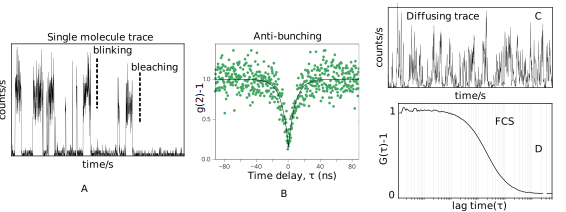
\includegraphics[width=\textwidth]{SM_characteristics}
	\caption{\textbf{Single-molecule characteristics.}
	(A) Time trace of a single molecule showing single-step switching (blinking) and bleaching.
	Notice the reappearance of the intensity after blinking but its irreversible disappearance after bleaching.
	(B) Anti-bunching at zero delay time in the correlation shows that the photons are emitted by a single emitter.\cite{chu2016a}
	(C) Time trace of diffusing molecules in a fluid with \SI{1}{\nM} fluorophores, showing intensity bursts and the large correlation amplitude ($G(\tau)-1={\sim}1$) indicating the presence of few molecules in the focus.}
	\label{fig:SM_characteristics}
\end{figure}

Fluorescence correlation spectroscopy (FCS) is often considered as a single-molecule technique. It measures the temporal correlation of fluctuating light intensities.\cite{magde1972thermodynamic,elson1974fluorescence,krichevsky2002fluorescence}
The conventional way to perform FCS is to collect the signal from \textit{diffusing fluorescent} molecules in the diffraction-limited focal volume and then to compute the autocorrelation of the intensity trajectory.
The autocorrelation of the intensity signal is given as $G(\tau)=<I(t)I(t+\tau)>/<I(t)>^2$ where I is the intensity, $\tau$ the lag time and $<...>$ represents time averaging.
The correlation quantifies the probability that the intensity at time $t$ is similar to the intensity at a later time $t+\tau$.
It provides information on the concentration and the time scale of the fluctuating observable.
By its very nature, FCS requires fluctuation of the number of diffusing fluorophores in the diffraction-limited volume of \SI{1}{fL}, preferably a number of the order of one molecule per focal volume on average.
Because of the diffraction limit ($\Delta{x}={\lambda}/2$), FCS is often limited to nanomolar and picomolar concentrations of the analyte. 

Two of the important requirements to measure single molecules with high spatial and temporal resolution are (i) high fluorescence yield and (i) small excitation and detection volumes.
In this thesis we push the limit of single-molecule detection to low quantum yield dyes and to a high concentrations of fluorophores.

\section{Time-Correlated Single-Photon Counting (TCSPC)}
Fluorescence signals are normally recorded as fluorescence intensity and are obtained by recording a photodiode voltage as a function of time.
The advancement in sensitive detectors enabled the detection of individual quanta of light, with single-photon counting units.
Detailed information about a single molecule can be extracted when all the photons detection events are registered in time.
The time-resolved technique used to record the information about photons is known as Time-Correlated Single-Photon Counting (TCSPC).\cite{oconnor2012timecorrelated,birch2002topics}
This technique requires a pulsed laser with high repetition rate (\SI{\sim80}{\MHz}) and a short pulse duration (picoseconds).
TCSPC is suitable for low signals with less than one photon on average per laser pulse.
With each laser pulse, there is a probability of excitation of the molecule which depends on the excitation cross section, and on the intensity of the laser.
Once excited, the molecule may emit a photon with a probability depending on the radiative and nonradiative rates of excited state relaxation.
The fluorescence lifetime can be given as:
\begin{equation}
	\tau_f = \frac{1}{\Gamma_{r} + \Gamma_{nr}}
\end{equation}
The arrival time of the emitted photon after the exciting laser pulse is called microtime (t\_micro) and the absolute arrival time from the start of the measurement called macrotime (t\_macro).
\begin{figure}
	\centering
	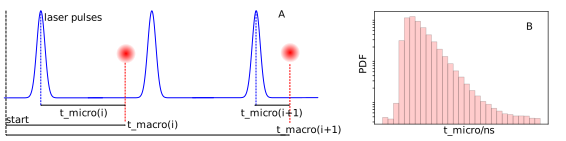
\includegraphics[width=\textwidth]{tcspc_sch}
	\caption{\textbf{TCSPC.} (A) The scheme of a time-resolved experiment showing the laser intensity trace (blue curve) and the subsequently detected photons as the red dots.
	The arrival time of emitted photons after the laser pulse is called microtime and the arrival date after the start of measurement is called macrotime.
	(B) The histogram of the micro-times gives the life time of the fluorophores.}
	\label{fig:tcspc_sch}
\end{figure}
The advantages of TCSPC measurements can be summarized as follows:
\begin{itemize}
	\item \textbf{Binning-free data.} As each photon is recorded with its arrival time, TCSPC is binning-free, unlike the intensity measurements.
	From the photon arrival time, intensity traces with any binning time can be reproduced after the measurement.
	The accessible dynamic range is limited at short times (picoseconds) by the resolution of the detector and the laser pulse duration, and for long times by the total recording time.
	Fluorescence correlation spectroscopy (FCS) utilizes the information provided by TCSPC and displays dynamics occurring over many orders of time in a single autocorrelation curve, often plotted on a logarithmic time scale.
	\item \textbf{Lifetime.} The distribution of photon delays after excitation (t\_micro) often follows a single-exponential distribution with an average fluorescence lifetime, which can be obtained by fitting the histogram of microtimes (Figure \ref{fig:tcspc_sch}B).
	Lifetime can not only give the intrinsic decay rate of the excited fluorophore, it also carries information about the immediate surroundings with which the dye interacts.
	Other applications of lifetime measurements are fluorescence resonance energy transfer (FRET) and fluorescence lifetime imaging.\cite{selvin2000the,lakowicz1992fluorescence} 
	\item \textbf{Linking of microtime and macrotime.} As each photon is stamped with microtime and macrotime, correlations can be extracted between the lifetime and dynamics of the macromolecules.
	Multiple fluorophores in a system can be distinguished on the basis of their fluorescence lifetimes.
\end{itemize}
In this thesis, almost every fluorescence measurement was done with both microtime and macrotime stampings.
In Chapter 2, both micro and macro times are used to distinguish the shorter lifetime photons from the longer lifetime photons to enhance the visibility of correlation in FCS experiments.
Chapter 3 utilizes the inter-photon times (t\_macro(i+1) - t\_macro(i+1)) to extract information that can be misrepresented by the binning methods.
In chapter 4, the potential of TCSPC is tested to explore dynamical heterogeneity in an electron-transfer protein. 
%
\section{Optical nano-antennas for single molecules}
Single-molecule fluorescence spectroscopy is usually limited to fluorophores with high quantum yield (\SI{>10}{\percent}) and to very low concentrations of molecules (\SI{}{\pM-nM}).
A large fraction of absorbing molecules including biomolecules and metal complexes show weak fluorescence with very low quantum yield (\SI{<1}{\percent}).
Background auto-fluorescence in physiological conditions often reduces the signal-to-noise ratio.
In addition, a majority of physiological reactions involving proteins and enzymes require milli- to micro-molar concentrations of substrates and cofactors.\cite{craighead2006future,punj2013gold,fabrizio2016roadmap,punj2014thesis}
Thus, systems at physiological conditions with micromolar concentrations cannot be studied conveniently by conventional single-molecule fluorescence microscopy.
Nano-plasmonics offer a promising solution to both these problems, by lifting the concentration limit by light confinement in the optical near field, and by enhancing the emission rate of dyes with poor fluorescence quantum yields.

Optical nano-antennas are similar to radio antennas at the macro scale.
Antennas are used to control and manipulate electromagnetic (EM) waves in the sub-wavelength scale.
Currents from a transmitter can be coupled to an antenna and radiated as EM wave to the far-field while on the other end EM waves in the far-field can be coupled to the antenna and sent to the receiver (Figure \ref{fig:nano_antenna}A,B).
Marconi used antennas with sizes of about ten meters antenna to control waves with kilometer wavelength. 
Similarly, nanoscale antennas can be used to control optical waves with sub-micrometer wavelengths. Nanoantennas present resonant modes called surface plasmon resonances (SPR's), involving collective motion of the metal's free electrons. Excitation of these surface plasmon resonances provide strong near-field enhancements, confining electromagnetic waves to local hot spot. \cite{bath8624,schuller2010plasmonics,ozbay2006plasmonics,maier2005plasmonics,hess2012active} In addition to the SPR effect, the local electric field is also enhanced by the lightning rod effect which is a result of the high charge density at the edges or sharply curved tips of the antennas.
Compared to the diffraction limit of light, or order $\lambda/2$, plasmonics can confine light down to much smaller spots, even less than nanometers in geometries with nanoparticles on a mirror\cite{benz2016singlemolecule}.
\begin{figure}
	\centering
	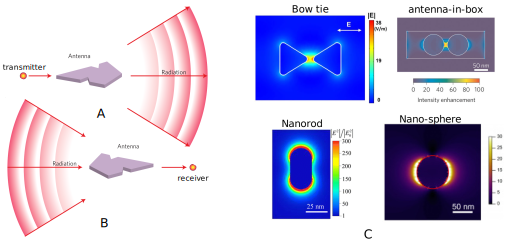
\includegraphics[width=\textwidth]{nano_antenna}
	\caption{\textbf{Optical nano-antenna.} Antenna coupled to the emitter (or transmitter, A) and receiver (B). The direction of energy flow is shown by the arrows.
	Antennas help convert free propagating light waves to localized energy and help radiate localized energy into the far-field.
	(C) Examples of nano antennas with their enhanced electric field.
	The color scales are indication of the electric field ($|E|$) or its intensity ($|E|^2$), as indicated close to each nano-structure.}
	\label{fig:nano_antenna}
\end{figure}
The fluorescence of an emitter placed in the near-field of a nano-antenna will be enhanced (i) by enhanced excitation in the high near field and (ii) by enhancement of the radiative decay rate.
Because of the high light intensity in the near-field, the fluorophore will be pumped harder. This effect is known as excitation enhancement.
The transition probability of an emitter governed by Fermi's Golden rule depends on the local density of states (LDOS) in addition to the transition matrix element between the two states.
Nano-antennas significantly modify the LDOS by enhancing the radiative rates of the emitter, leading to increased spontaneous emission. This effect known as radiative enhancement.
Close to the metal surface, additional non-radiative channels lead to quenching of fluorescence via Ohmic losses.
Thus the resultant enhancement depends upon the emitter's position and orientation with respect to the antenna, and on the overlap of its emission spectrum with the resonance of the antenna.\cite{anger2006enhancement,khatua2014resonant}

The strength of the field enhancement and the field spatial distribution depend on the nanostructure, as shown in the examples of Figure \ref{fig:nano_antenna}C.
The quality of an antenna is judged by the large field enhancement factor and smaller mode volume.
Bow tie antennas and antennas-in-box provide high field enhancements and small near-field volumes but require tedious and expensive lithographic expertise.\cite{novotny2011antennas,regmi2017thesis}

A gold nano-sphere is the most straightforward example of a nano-antenna, but it gives low field enhancement and large near-field volume.\cite{punj2013gold}
Gold nanorods are somewhat better antennas because of their larger field enhancement and somewhat larger field confinement compared to nanospheres. Morover, they present a stronger and narrower spectral response than spheres. For this thesis, gold nanorods are our favorite nano-antennas because:
\begin{itemize}
	\item Their field enhancement is comparable to that of the best antennas available.
	\item The plasmon resonance can be tuned from green to far-infrared simply by changing the aspect ratio of the rod.\cite{link1999simulation}
	The spectral width of the plasmon is relatively small and the confinement volume can be controlled to some extent by changing the volume of the rod.
	The narrow surface plasmon resonance is helpful for selective enhancement of emitters.\cite{yuan2013thousandfold,khatua2014resonant}
	\item Gold nanorods can be cheaply mass-produced by colloidal synthesis with high crystalline quality and smooth surfaces.\cite{nikoobakht2003preparation,perezjuste2005gold}
	\item Accessibility. As nanorods are small and colloidal in nature, they can be easily inserted into living cells.
	In fact, because of their photoluminescence, they are already being used in living cells or tissues for imaging.
	\item Selective reactivity. Gold is inert and harmless for living organisms unlike other metals like silver.
	It has high affinity towards thiols opening the possibility of chemical functionalization.
\end{itemize}
%
\section{Proteins at work are proteins in motion}
Proteins and enzymes are the machines inside living cells that perform all vital functions, including mechanical work and energy maintenance.
Proteins and enzymes are often pictured by their static structures obtained by crystallography or the average structure of a large ensemble of conformations obtained from NMR spectroscopy.
The functions of a protein are governed by its dynamical motions. A multidimensional energy landscape and different kinetic barriers govern the complex coordinated motion of proteins. Understanding how protein function is related to structure and dynamics, we need to follow their physical properties in the fourth dimension, time. Enzymes perform chemical reactions by binding with their substrate and minimizing the energy barrier which needs to be overcome for product formation.
Spectroscopic studies done in the 1980's and recent nuclear magnetic resonance (NMR) investigations show the amplitude and duration of structural fluctuations involved in the function of enzyme catalysis and protein function.
Movements are observed on time scales ranging from picoseconds corresponding to atomic movements to milliseconds involving movement of bigger domains.\cite{henzler-wildman2007dynamic,frauenfelder1991the}
The time scale of transitions relates to the energy barriers between different conformations. Those are represented as a free-energy landscape of a multidimensional space of reaction coordinates.
The concept of energy landscape was first introduced by Frauenfelder and co-workers\cite{frauenfelder1991the} to explain the observation of multiple energy barriers and non-exponential kinetics in the rebinding of carbon monoxide and oxygen to myoglobin.
They connected the myoglobin function to the energy barriers and the existence of conformational sub-states.
Since then, other studies by NMR and single-molecule techniques have advanced our knowledge about the details of protein energy landscapes.

\begin{SCfigure}[0.9][ht] %this figure will be at the right
    \centering
    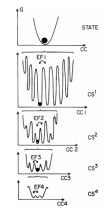
\includegraphics[width=0.4\textwidth]{energy_landscape}
    \caption{\textbf{Hierarchical arrangement of the conformational substates.} The energy landscape of a protein shows hierarchical protein dynamics and energy barriers. The upper diagram shows an energy minimum representing a state of the protein. Zooming in on that state, we find more substates, which themselves subdivide into more and more conformational substates at higher and higher order of energy. Up to four tiers can been defined in the hierarchy of conformational substates.}
    \label{fig:energy_landscape}
\end{SCfigure}

An energy landscape is defined as a map of all possible atomic positions in a molecule and their corresponding Gibbs free energy.
The very complex multidimensional energy landscape is typically represented in a two-dimensional conformational coordinate (cc) system.
The hypersurface of energy landscape consists of a number of valleys. Each free-energy minimum corresponding to the initial and final state of a reaction is called a ``state'' while each saddle point between two minima is known as a ``transition state''.
Each state can assume a very large number of conformational substates, which can be hierachically ordered into different tiers of energy (Figure \ref{fig:energy_landscape}).
The transition time directly relates to the energy barriers, the transitions in the tier-4 ($CS^4$) occurs in a faster time scale than in the tier-0($CS^0$).
Protein motions can be categorized mainly into two types- equilibrium fluctuations (EF) and  functionally important motions (FIMs).\cite{ansari1985protein}
EFs involve motions among the substates and result in equilibrium thermodynamic properties like entropy and internal energy. 
Examples of equilibrium fluctuations include bond vibration, methyl rotation, loop motion and side chain conformational changes. Larger changes in the structure during functionally important movements may bring the protein to different substates. Any reaction whose rate depends on the conformational substate will thus exhibit rate fluctuations, leading to non-exponential kinetics and dynamical heterogeneity. In this thesis, we will investigate the rate of complex formation between an electron transfer protein and its redox partners. We will attribute variation in the rates, i.e. the dynamical heterogeneity, to conformational changes.

\section{Azurin: An Electron Transfer Protein}
Electron transfer via oxidation and reduction controls vital cellular processes like respiration, redox homeostasis, photosynthesis, to name a few.
Proteins with a metal co-factor play a crucial role in carrying out such electron transfer.
Among the metalloproteins, Copper and Iron proteins are most common. They carry out various activities, like oxygen transport (hemocyanin), respiration (cytochrom-c oxidase) and metal homeostasis (ceruloplasmin).
Because of their electron transport properties, metalloproteins are promising candidate for biosensors and biomolecular electronic devices.

Azurin is a copper-containing protein involved in electron transfer in cells.\cite{dennison2005investigating,kolczak2006handbook}
The Copper ion is buried in the so-called northern side of azurin (MW=\SI{14}{\kilo\dalton}). It is surrounded by a coordination sphere composed of two histidines, a cysteine and methionine\ref{fig:azurin_structure}.
The copper atom in azurin can possess either of the two oxidation states: Cu(II) and Cu(I).
Cu(II) azurin has a blue color due to the absorption at \SIrange{595}{630}{\nm} arising from $\pi - \pi^*$ transition in the molecular orbital scheme of azurin.\cite{dooley1981spectroscopic,schmauder2005sensitive}
In contrast, Cu(I) azurin is colorless as it has no absorption band in the red(Figure \ref{fig:flurox_azurin}.
The different spectroscopic characteristics of the two states of Cu can be used to measure the kinetics of electron transfer of azurin.
The oxidation and reduction reactions via electron transfer are generally known as redox reaction.
The redox properties of azurin are determined by the Cu atom and the ligands surrounding Cu.
Azurin has a midpoint potential of \SI{60}{\mV}(vs Saturated Calomel Electrode, SCE) at pH 7.
Azurin is well characterized and is a reasonably stable protein at room temperature which makes it a suitable candidate for investigating fundamental properties of electron transfer reactions.
\begin{figure}
	\centering
	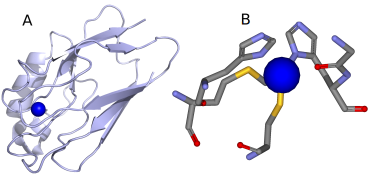
\includegraphics[width=\textwidth]{azurin_structure}
	\caption{\textbf{Azurin structure.} (A) Crystal structure (cartoon representation) of azurin from \textit{Pseudomonas aeruginosa}.\cite{adman1981structural}
	The Copper atom is shown as a blue sphere.
	(B) Ligands around Copper atom: His117, His46, Cys112, Met121}
	\label{fig:azurin_structure}
\end{figure}

\section{Fluorox Principle (FRET-redox)}
The absorption band at \SIrange{595}{630}{\nm} of azurin has been used to study electron transfer kinetics in ensembles.
To study electron transfer in single azurin molecules, a more sensitive background-free fluorescence-technique in the red-infrared range can be used.
The external fluorescent marker ATTO655 is attached, as azurin doesn't have intrinsic fluorescence in the red spectral range.
If the emission spectrum matches (see Figure~\ref{fig:flurox_azurin}) with absorption of Cu(II) azurin, the dye fluorescence will be quenched in the oxidized state, whereas the fluorescence in Cu(I) will be bright due to the absence of quenching.
In other words, the oxidation state of the azurin can be read out simply by looking at the fluorescence of labeled azurin.
The principle to detect the oxidation state in metalloenzymes by looking at the fluorescence of an external marker is called FluoRox. It was pioneered by Aartsma and co-workers.\cite{kuznetsova2008the,goldsmith2011redox,tabares2011fluorescence}
\begin{figure}
	\centering
	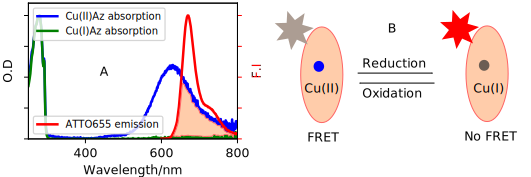
\includegraphics[width=\textwidth]{flurox_azurin}
	\caption{\textbf{Fluorox principle.} (A) Spectral overlap between the absorption of azurin and the emission of ATTO655. Blue curve: absorption of Cu(II) azurin, green: absorption of Cu(I) azurin, red: emission of ATTO655.
	(B) Symbolic representation of the fluorescent state of azurin-ATTO655 in Cu(II)-state and Cu(I) state. In the Cu(II) state, copper is shown as a blue sphere and the non-fluorescent ATTO655 is shown in light gray. In the Cu(I) state, copper is shown in green and the fluorescent ATTO655 is shown in red.}
	\label{fig:flurox_azurin}
\end{figure}
The efficiency of fluorescence quenching can be calculated as in fluorescence resonance energy transfer (FRET). It is given by:
\begin{equation}
	E = \frac{R_0^6}{R_0^6 + r^6}	
\end{equation}
$r$ is the distance between the Cu-atom and the dye, and $R_0$, called the $F\ddot{o}rster$ radius, is the distance at which the efficiency is \SI{50}{\percent}. 
$F\ddot{o}rster$ can be given as:
\begin{equation}
	R_0 = 0.211[\kappa^2n^{-4}Q_DJ(\lambda)]^{1/6}	
\end{equation}
where $\kappa^2$ is an orientation factor, n the refractive index of the solvent, $Q_D$ the quantum yield of the donor and $J(\lambda)$ the spectral overlap between the absorption of azurin and the emission of the dye.
The overlap between the emission of the dye ATTO655 and the absorption of azurin can be visually seen in Figure~\ref{fig:flurox_azurin}A.
When ATTO655 is attached at the Lys122 of azurin, the quenching efficiency is around \SI{90}{\percent}.
Such high quenching efficiency of Lys122 labeled azurin allows us to study electron transfer and its heterogeneity at the single-molecule level(Chapter~5).

\section{This thesis}
The common theme of this work is single-molecule fluorescence. In the first part of the thesis, we try to improve signals from single molecules by plasmonic fluorescence enhancement, and to characterize the near field of the plasmonic structures from the statistics of enhanced signals. In the second part, we use the potential of single-molecule microscopy to gain insight into changes of conformational substates, by looking at the electron transfer dynamics in azurin.

\begin{itemize}
	\item \textbf{Chapter 2.} Many physiological reactions like enzyme-substrate reactions occur in millimolar to micromolar concentrations. Single-molecule studies do not provide direct access to such a high concentrations because there are still thousands of molecules in the diffraction-limited detection volume of few femtoliters. In this chapter, we use gold nanorods to perform fluorescence correlation spectroscopy at physiologically relevant concentrations. The gold nanorod helped to confine light to smaller volumes and enhance the dye fluorescence. The fluorescent probe molecules (ATTO647N) were allowed to freely diffuse in a supported lipid bilayer. The zwitterionic head groups on the lipid prevented any non-specific interaction with the substrate and the gold nanorod. Similar diffusion coefficients were observed in the far-field and near-field suggesting the absence of influence of the gold nanorod on the dye diffusion. The diffusion times in the near-field and far-field allowed us to determine the extent of the near field of the gold nanorod. The fluorescence of the dye was enhanced by a maximum factor of five. The lower enhancement factor was attributed to the inaccessibility of the diffusing dyes to the hottest spot in the near field and to the high quantum yield of the probe (\SI{70}{\percent}).
	The enhanced dyes had a shorter lifetime than the un-enhanced dye. By filtering out photons with longer lifetime, the correlation contrast was improved by more than two orders of magnitude. We also functionalized the bilayer with azurin-ATTO655 (biomolecule) and obtained similar improvement in the correlation contrast without any nonspecific interaction with the substrate.

	
	\item \textbf{Chapter 3.} The fluorescence enhancement factor by a single plasmonic structure varies strongly  (up to three orders of magnitude) depending on the position and orientation of the fluorescent probe. Furthermore, fluorescence bleaching limits the number of single molecules to one per single nanorod (in single-molecule study). In this chapter we use transient binding by DNA to repeatedly and reproducibly study many single molecules on a single nanorod on the same spot on its tip. The longer persistence length of DNA helps to keep the dye at a fixed distance from the tip. We optimized the passivation of the gold nanorod surface to control the average number of binding sites, down to one and to minimize fluctuations of intensity of enhanced fluorescence.

	\item \textbf{Chapter 4.} A more general way to characterize single-molecule time traces is to bin the trace and look for histograms of intensities and durations of the transitions. The enhancement factor extracted from the time traces in the presence of a gold nanorod were different for different binning times. We investigated the interphoton times to extract an average enhancement factor and the number of molecules in the near field. We performed numerical simulations and theoretical models to extract the intensity distribution for slowly diffusing molecules in a two-dimensional bilayer. The non-exponential character of the interphoton time distribution was found to strongly depend on the average number of molecules in the near field. Work is in progress to investigate enhanced fluorescence histograms in the presence of molecular diffusion.

	\item \textbf{Chapter 5.} In this final chapter, we investigated electron transfer in redox active single azurins. The oxidation state of the Cu-azurin was read out by observing the brightness of the fluorophore. Switching of Copper oxidation state was studied at different redox potentials where the potential was controlled electrochemically by a potentiostat. The distribution of midpoint potentials was characterized both spatially and dynamically (longer time traces). The rate of complex formation between azurin and its redox partners showed correlated variations in time. As the variations were observed in steady state conditions and on a passive functionalized glass surface, the heterogeneity was attributed to the different conformation (substates) of azurin.
\end{itemize}
% \references{bibliography}=
% \chapter{Gold-nanorod Enhanced Fluorescence Correlation Spectroscopy(EFCS) on a lipid bilayer(SLB)}
\label{chapter:EFCS}
%!TEX root = ../thesis.tex
% \blfootnote{This chapter have been published in J. Phys. Chem. C 2016, \textbf{120}, 25996−26003}

\section{Introduction}
\section{Method}
\section{Result and discussion}
\subsection{Fluorescence enhancement}
\subsection{Lifetime as additional identifier of enhanced signal}
\subsection{FCS and contrast improvement}
\subsection{EFCS with biomolecules}
\section{conclusion}
% \references{bibliography}
% \chapter{Binned and bin-free analysis of Fluorescence Enhancement by gold nanorod on a 2D layer}
\label{chapter:binfree}
\graphicspath{{./chapters/c3_binfree/figures/}}
%============================ MAIN ================================

\begin{abstract}
Gold nanorods are extensively used for single-molecule fluorescence enhancement as they are easy to synthesize, bio-compatible and provide high light confinement at their nanometer-sized tips. The current way to estimate fluorescence enhancement relies on binned time traces or on fluorescence correlation spectroscopy (FCS). We report on novel ways to extract the enhancement factor in a single-molecule enhancement experiment, avoiding the arbitrary selection of one or a few high-intensity burst(s). These new estimates for the enhancement factor make use of the whole distribution of intensity bursts, or of the interphoton delay distribution, which avoids the arbitrary binning of the fluorescence intensity time traces. We present experimental results on the bi-dimensional case, experimentally achieved using a lipid bilayer to support the diffusion of fluorophores.  We support our findings with histograms of fluorescence bursts and with an analytical derivation of the interphoton delay distribution of (nearly) immobilized emitters from the fluorescence intensity profile.
\end{abstract}
\newpage
%============================ Introduction =====================================
\section{Introduction}
Single quantum emitters such as fluorophores, quantum dots, color centers 
and fluorescent proteins have become powerful tools for modern science 
since they provide nanometer-sized probes that can be used to extract 
information about the local environment \cite{moerner1999illuminating, kulzer2010single}, 
oxidation state of molecules \cite{zhang2017gold} and proximity of other 
emitters using F\"oster resonance energy transfer (FRET) \cite{jares2003fret,stein2011single,kalinin2012toolkit}. 
These unique advantages are joined to those of non-invasive optical methods. 

%-Fluorescence enhancement by plasmonic structures paragraph: physical origins, dependence, mention emission and excitation. limitations. motivate the quantification of enhancement in different structures.
Fluorescence enhancement by plasmonic nanostructures has been successfully 
used in the past to increase the signal from weak 
emitters \cite{kinkhabwala2009large, yuan2013thousandfold, khatua2014resonant} even in 
living cells \cite{vanzanten2010imaging}. In a nutshell, fluorescence enhancement
by metallic nanoparticles refers to a considerable increase in the rate of detected 
photons whenever a (often weakly) fluorescent molecule is placed in the vicinity of the nanoparticle.
Enhancement heavily relies on the surface plasmon resonance of the nanoparticle, which often lies
in the optical spectral range. When excited at this resonance frequency, 
the nanoparticles can concentrate optical fields in tiny volumes,
the so-called ``hot spots'', providing a sub-diffraction 
working volume that can be exploited to extend the powerful technique fluorescence 
correlation spectroscopy (FCS) to micromolar 
concentrations \cite{estrada200810000,manzo2011nanoscale,kinkhabwala2012fluorescence,punj2013gold,khatua2014enhancedfluorescence}. 
Notably, this approach was also used to study molecular diffusion in the membrane 
of a living cell \cite{flauraud2015largescale}.
Fluorescence enhancement also provides a way to extend the powerful tools of single-molecule spectroscopy to 
weakly emitting species.


Regardless of the origin of the fluorescence photons, a usual approach is to record the arrival time of each individual 
photon in the so-called time-correlated single-photon counting (TCSPC) approach in a time-tagged 
time-resolved (TTTR) configuration  \cite{Wahl_picoquant,becker2015advanced}. 
Thanks to the high-speed electronics and pulsed excitation sources available commercially, 
the absolute arrival times (also called macrotimes) can be determined with picosecond accuracy and, with the proper synchronization to the excitation source, the ``nanotimes'' \footnote{The usual denomination is microtime but we opt for nanotime to avoid confusion with the macrotime.} can be also determined. 
The nanotime is usually used to obtain the lifetime histogram, which can be used to 
gain insight into the underlying mechanism of the emission. For example, 
in the case of fluorescence, the radiative and non-radiative rates can be accessed experimentally with a 
measurement of the lifetime if the quantum yield is known \cite{lakowicz2007principles}.
%Figure \ref{fg:tcspc} shows an time representation for such an experimental configuration. 
The output of a TTTR experiment can be represented as a classical function of time \cite{Lippitz2005}:

\begin{equation}
I(t) = \sum_i \delta( t-t_i)
\label{eq:intensity_TCSPC}
\end{equation}
where $\delta(t)$ is the usual Dirac function and $t_i$ is the absolute arrival time
for each detected photon in the experiment (measured relative to the start of the experiment, the macrotime). 
We shall call this function \textit{unbinned time trace}. 
 

 %\begin{figure}
 %\includegraphics[width=\textwidth]{img/TCSPC_scheme.pdf}%
 %\caption{\textbf{Time-correlated single-photon counting detection scheme.} Typical configuration for a time-tagged time-resolved photoluminescence experiment. The exciting source is a pulsed laser with MHz repetition rate and both the time tag $T$ since the start of the experiment and the TCSPC time $t$ are recorded and saved. The former can be used to calculate the interphoton delay distribution and the latter to generate a lifetime histogram to obtain, for example, the lifetime of a fluorescent molecule. Modified from \cite{Wahl_picoquant}.
%\label{fg:tcspc}}
 %\end{figure}

In spite of the high temporal resolution provided by such experiments, 
the usual way to characterize the emission of quantum emitters is to 
display the time trace of the number of detected photons 
in a certain integration time (or binning time) and to
complement this with a histogram of detected photon counts per time bin. 
Such a characterization inherently introduces an arbitrary parameter, 
the binning or integration time, that may bias the obtained distribution \cite{Lippitz2005}. 
Alternatively, correlation functions can be calculated from the unbinned
 time trace to exhibit the characteristic 
time of a process of interest, such as the diffusion \cite{magde1972thermodynamic,haustein2007fluorescence} 
or rotation \cite{loman2010measuring} characteristic times of molecules in solution as well as 
other molecular properties even at single-molecule level \cite{medina2002fluorescence, ghosh2017quantifying}.
This approach can provide estimates of the enhancement factor, but is very sensitive to 
background corrections \cite{pradhan2016goldnanorodenhanced, langguth2014simple}. 
The common practice to determine fluorescence enhancement is to screen the time trace 
for the strongest fluorescence burst(s), corresponding to unlikely event(s) that a 
molecule occupies the best position in the hot spot of the plasmonic near field for 
a long enough time. This procedure, often nicknamed ``cherry-picking'', depends on the 
binning time, on the diffusion constant, and on the stochastic character of each 
molecule's trajectory. There is no warranty that waiting for longer times, or binning 
at higher resolution, wouldn't lead to larger enhancement factors. Therefore, there 
is a pressing need for less arbitrary ways to quantify the enhancement factor. 

Here, we focus on the use of a less common quantity, the 
\textit{interphoton delay distribution} $p(\tau)$,
to characterize the emission of quantum emitters and to extract reliable 
information about an emitting system avoiding the introduction of any arbitrary 
binning time. The interphoton delay distribution expresses the delay distribution 
between consecutive photons: after each photon detection, the probability density to observe 
the next photon at a time $\tau$ is $p(\tau)$ ($p(\tau)\geq 0$) \cite{Verberk2003}.
Experimentally, it can be obtained by simply plotting a histogram of the time differences between 
successively detected photons.

In this paper we present a model to relate the interphoton delay distribution
to the spatial distribution of fluorescence intensity delivered by a 
single quantum emitter in the limit of \textit{slow} diffusion. We show that $p(\tau)$ 
encodes information about the intensity distribution inside the volume accessible 
to diffuser. We will illustrate this point with single-molecule fluorescence 
in a bi-dimensional case both with a Gaussian beam shape and with addition of a power-law model of 
enhanced fluorescence by a gold nanorod. 
Furthermore, we propose to use the interphoton delay distribution to estimate
the enhancement factor in fluorescence enhancement experiments, avoiding
arbitrary parameters such as a binning time. 

This paper is organized as follows. First we present a theoretical
derivation of the interphoton delay distribution in Sec. \ref{sec:teo}. In Sec.
\ref{sec:TB}, we compare the experimental and theoretical results in
the simple case of an emitter switching between two intensity levels. Then, in Sec. 
\ref{sec:gaussian2d}, we move to the 
more complex case of two-dimensional diffusion of molecules under excitation by a
Gaussian beam, where our model captures the essence of the process.
In Sec. \ref{sec:model_enha} we present a simplified model for the
enhancement from a single nanoparticle, using the interphoton delay distribution
to characterize the phenomena. 
Finally, in Sec. \ref{sec:enhancement} we analyze experimental data and 
compare enhancement factors obtained by the 'cherry-picking' procedure and the 
other estimates provided by the interphoton delay histogram and by a statistical burst analysis.

\section{Theoretical framework\label{sec:teo}}

We seek to relate the interphoton delay distribution in a fluorescence experiment with 
the spatial distribution of intensities used to excite the fluorescent molecules. The interphoton
delay distribution defined above is represented by the probability density function $p(\tau)$. 
Thus the probability of detecting the next photon between times $\tau$ and 
$\tau+\mbox{d}\tau$ is $p(\tau)\mbox{d}\tau$ and the
normalization condition holds: $\int_0^{\infty}{p(\tau)\mbox{d}\tau}=1$.

Let us start from the simplest case of a constant detected intensity $w$ 
(in counts per second). Such a signal gives rise to exponentially distributed 
interphoton delay times, i.e., 
\begin{equation}
p(\tau)=w\exp(-w\tau)\,.
\label{eq:exponential_distribution}
\end{equation}
This is a direct consequence of the memory-free character of the photon 
emission, which leads to a Poisson distribution of the number of photons 
emitted per binning time and to an 
exponential distribution of interphoton delays. We note that this distribution 
can be obtained with a fluorescent molecule excited at a constant intensity, 
for example, a fixed molecule immobilized on a substrate. 

Let us now consider the limit of very slow diffusion. Variations in the local 
intensity seen by an individual emitter are much slower than delays between 
photon detection events, so that there arises a distribution of intensities 
$Q(w)$ corresponding to various spatial configurations of emitters in and 
around the excitation focal spot.
Averaging over this distribution of intensities gives rise to the interphoton 
delay distribution $p(\tau)=\int_0^\infty w e^{-w\tau}Q(w)\mbox{d}w$, which 
corresponds to over all possible intensities (rates) $w$ and can be rewritten as

\begin{equation}
p(\tau)=-\frac{\mbox{d}}{\mbox{d}\tau}\mathscr{L}\{Q\}(\tau)\,,
\label{eq:interphoton_delay_distribution}
\end{equation} 
where $\mathscr{L}\{Q\}(\tau)=\int_0^\infty e^{-w\tau}Q(w)\mbox{d}w$ denotes the 
Laplace transform \footnote{Note that the Laplace transformation
is usually applied to time-dependent functions, giving rate-dependent functions. 
Here, we apply it to a function of the rate and thus obtain a time-dependent transform.} of the function $Q(w)$. 
If we seek the interphoton delay distribution 
corresponding to the added signals of two sources with intensity distributions $P(w)$ 
and $Q(w)$, we can use the total intensity $T(w)$ that can be calculated as the sum 
of a combined probability of source 1 emitting at a rate $x$ and source 2 at a rate 
$(w-x)$, i.e., by convoluting the two intensity functions: $T(w)=\int{P(x)Q(w-x)\mbox{d}x}$. 
Using the convolution theorem we can write the Laplace transform of the intensity distribution 
as the product of the Laplace transforms of the two distributions, from which we can deduce 
the interphoton delay distribution.

Let us now consider as a source one point-like emitter at position $\ve{r}$, for example, a fluorescent molecule
diffusing around an optical intensity maximum. 
The detected intensity will generally be a product of the position-dependent local 
excitation intensity and of a position-dependent collection efficiency, with some 
molecular parameters involved in the fluorescence process (absorption cross section, 
fluorescence quantum yield, etc. ). We write the product of these factors as a 
position-dependent fluorescence intensity profile $I(\ve{r})$. 

At this point we stress two important approximations in our model. The first one is 
to neglect rotational diffusion of the molecules, which is a good approximation 
if we study times that are much longer than the rotational diffusion time. The 
second important approximation is to assume that translational diffusion is slow
 compared to the photon detection rate, i. e., the molecules are nearly fixed 
during the emission process. A complete theory relaxing this approximation would 
be much more complicated and exceeds the scope of this work.

Under these approximations, the photon distribution can be deduced from the 
intensity distribution. Exploration of the diffusion volume $V$ accessible to the moving emitter gives rise to the following distribution of intensities 
\begin{equation}
Q_1(w)=\frac{1}{V}\int_V{\delta\left( w-I(\ve{r})\right)\mbox{d}^3r} \,,
\label{eq:intesity1}
\end{equation} 
where $\delta(x)$ represents the Dirac delta function. To calculate the interphoton delay 
distribution using Eqn. (\ref{eq:interphoton_delay_distribution}), we need the Laplace transform of $Q_1(w)$, 
\begin{equation}
\mathscr{L}\{Q_1\}(\tau) = 1 -\lambda(\tau) \quad \mbox{where} \quad 
\lambda(\tau)\equiv \frac{1}{V}\int_V{ \{1-\exp[-I(\ve{r})\tau]\}\mbox{d}^3r} \, .
\label{eq:lambda}
\end{equation} 
Note that, for an intensity variation with a finite range around the center, 
for example due to Gaussian illumination and/or collection, $\lambda(\tau)$ is a 
small quantity which tends to zero for a large diffusion volume.  

We now consider the case of many ($N$) emitters with a concentration $C={N}/{V}$
 diffusing in a large volume. Using the argument presented before for two emitters, 
the addition of one emitter will modify the intensity distribution by convolution 
with the one-emitter distribution function $Q_1(\tau)$. Using the convolution theorem 
for the Laplace transform, we can write the Laplace transform for the $N+1$ diffusers as
\begin{equation}
\mathscr{L}\{Q_{N+1}\}(\tau) = \mathscr{L}\{Q_N\}(\tau) \mathscr{L}\{Q_1\}(\tau)\,,
\label{eq:laplace_N}
\end{equation}
from which we deduce 
$\mathscr{L}\{Q_{N}\}(\tau)=\left[\mathscr{L}\{Q_{1}\}(\tau)\right]^N $. 
Now we apply the statistical method of Stoneham \cite{STONEHAM1969, fleury1993} 
by letting number and volume tend to infinity keeping the ratio constant to match 
the concentration $C$, and obtain:
\begin{equation}
\ln\left[\mathscr{L}\{Q_{N}(w)\}(\tau)\right] = 
N\ln\left[1-\lambda(\tau)\right] \approx - C V \lambda(\tau)\,.
\label{eq:stoneham_approx}
\end{equation}

Therefore, using this result in Eqn. (\ref{eq:interphoton_delay_distribution})
together with the definition from Eqn. (\ref{eq:lambda}), we find the histogram of 
interphoton delays for a concentration $C$ of emitters diffusing 
in a fluorescence intensity profile described by $I(\ve{r})$: 
\begin{equation}
p(\tau)=-\frac{\mbox{d}}{\mbox{d}\tau}\left[ 
\exp\left(-C \int_V{\left(1-\exp\left[-\tau I(\ve{r})\right] \right)}
\mbox{d}^3\ve{r}    \right)\right]\,.
\label{eq:result}
\end{equation}

This is a general result that allows us to calculate the interphoton 
delay histogram  for a solution with a concentration $C$ of slowly 
freely-diffusing objects in a fluorescence intensity profile $I(\ve{r})$. 
We note that the general result above fulfills the normalization condition 
for $p(\tau)$, as required for any probability density function.


%\subsection{Limit of infinitely fast diffusion}

The case of infinitely fast diffusion of the emitters is easily obtained by letting the concentration $C$ go to infinity and the intensity $I(\ve{r})$ vanish, while keeping their product, i.e., the total brightness per unit volume, constant. It is easily seen that the limit of Eqn. (\ref{eq:result}) becomes a single exponential distribution with an average intensity $W$:
\begin{equation}
W = C \int_V{I(\ve{r})\mbox{d}^3\ve{r}}\,.
\label{eq:intensity2}
\end{equation} 
This result is easily interpreted: in the fast diffusing case, each volume element contributes a constant intensity. Because the total intensity is constant, there are no intensity fluctuations and the distribution of delays is single-exponential. In other words, deviations from an exponential distribution of delays characterize fluctuations in the fluorescence intensity, themselves related to fluctuations of the number of emitters in the excitation volume. Just as in FCS, these fluctuations become more and more important as the concentration is lowered.


%It is interesting to study the the limit case of extremely fast diffusion, opposed 
%to the slow diffusion case presented previously. We assume a molecular concentration 
%$C_0$ and an intensity profile $I_0(\ve{r})$, and we aim to obtain the interphoton 
%delay distribution when the diffusion coefficient $D$ is large. This limit situation 
%is equivalent to a very small intensity at high concentrations, thus we take $C=C_0/\epsilon$
%and $I(\ve{r})=I_0(\ve{r})/\epsilon$ with $\epsilon \ll 1$.
%We start from equation \ref{eq:result} that can be rewritten as 
%
%\begin{eqnarray}\label{eq:result2a}
%p(\tau) & = & -\frac{\mbox{d}G(\tau)}{\mbox{d}\tau} \\
%\mbox{where}\,\, G(\tau) & \equiv & \exp\left(-C \int_V{\left(1-\exp\left[-\tau I(\ve{r})\right] \right)}
%\mbox{d}^3\ve{r}    \right)\, .
%\label{eq:result2b}
%\end{eqnarray}
%
%We expand to first order the  integrand in the last expression to obtain
%
%\begin{equation}
%\ln(G(\tau)) = -\frac{C_0}{\epsilon}\int_V \tau \epsilon I_0(\ve{r}) \mbox{d}^3\ve{r} 
%= -C_0 \tau \left< I_0 \right>_V\,,
%\end{equation}
%where $\left< I_0 \right>_V$ represents the mean intensity in the volume $V$. 
%By replacing this result in equation \ref{eq:result2a} we get a single exponential function
%for the interphoton delay distribution:
%
%\begin{equation}
%p(\tau) = C_0\left< I_0 \right>_V \exp\left( -C_0 \tau \left< I_0 \right>_V \right)\quad (D \rightarrow \infty)\,.
%\label{eq:d_inf}
%\end{equation}
%
%The molecules diffuse so fast that the fluctuations are averaged out and the curve we obtain is equivalent 
%to a single intensity value $w=C_0\left< I_0 \right>_V$ (see equation \ref{eq:exponential_distribution}).


\section{Two-state emitter \label{sec:TB}}
%
In order to show that we can avoid the binning of our TTTR data to 
extract valuable information about our experiment, we studied the 
simple case of an emitter switching between two fixed detected intensities. 
In such a scenario, and for slow enough switching,
the interphoton delay distribution will be a bi-exponential function.

\begin{figure}
\includegraphics[width=0.99\textwidth]{01_Figure_1_Transient_scheme}%
\caption{\textit{\textbf{Transient binding experimental scheme.} We used a 
home-made confocal microscope to excite and detect the imaging 
strand-Cy5 constructs in the solution. The signal from the molecules 
in the solution is low, thus we enhance the fluorescence signal using 
immobilized gold nanorods on a glass surface (average size: $45\times90 \,\mbox{nm}$). 
In order to experimentally access the same spatial position in the plasmonic 
hot spot we use a transient binding technique with a $15$-base pair 
DNA as the docking strand and a $10$-base pair complementary labeled DNA as the imaging strand. 
The docking strand is attached to the gold nanorod surface using 
two thiol bonds. } 
\label{fg:TB} }
\end{figure}

%
We experimentally access this situation by using fluorescence enhancement
by individual gold nanorods. In this scenario, 
a 1000-fold intensity enhancement can be achieved for weak 
dyes\cite{yuan2013thousandfold,khatua2014resonant}. However, this enhancement value
depends strongly on the position of the molecule in the nanoscale plasmonic 
hot-spot of the structure \cite{khatua2014resonant}, thus the challenge in 
such experiments is to place the dye molecules in the desired position to 
achieve high enhancement values. An elegant solution to place the molecules 
in the desired position is the technique called transient binding \cite{acuna2012fluorescence}.
Briefly, we use two complementary single-stranded DNA sequences, one attached
to the surface of a gold nanorod and the other, diffusing one, marked with a single Cy5
molecule (fluorescence quantum yield 0.27). The strand attached to the gold 
surface is called the docking strand, since it allows the complementary strand 
to dock in one specific site and the latter is called the imaging strand since 
it allows fluorescence detection. 

This experimental scheme is shown in Fig. \ref{fg:TB}. We immobilized 
a gold nanorod on a glass surface and the imaging strands diffuse 
freely in the buffer solution. %Details of the sample preparation can be found 
%in the Supplementary Information. 
When an imaging strand diffuses close to the 
docking strand, the DNA can hybridize, forming a temporary double strand DNA. 
In that scenario, the single fluorescent label is placed in the plasmonic 
hot spot of the nanorod and gets enhanced, giving a higher signal than the 
other molecules in the detection volume. 
This approach allows us to put a single dye in a well-defined position in the 
near field of the nanorod for an exponentially distributed time whose 
mean value can be controlled with the length of the DNA and the 
environment conditions \cite{jungmann2010single}. Since the dye molecule is fixed at a 
certain point in space, with a fixed exciting intensity, we expect a 
fixed detected intensity. The main advantage of this experimental 
approach is that the hybridization is transient and after some time 
the DNA will de-hybridize, freeing the docking site for another 
imaging strand to come. As a result, photobleaching of the dye 
is not a limiting factor for the experiment, since \textit{the same point} 
in space can be probed several times with different single molecules.

\begin{figure}
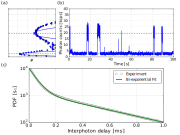
\includegraphics[width=0.95\textwidth]{02_Figure_2_transient_single_site_results}%
\caption{\textit{\textbf{Fluorescence enhancement of single Cy5 molecules with transient binding.}
(a) Binned intensity histogram (squares) with a fit with two Poisson distributions (blue lines). 
(b) Binned fluorescence time trace (bin time = $10\,\mbox{ms}$). 
From these two plots, two intensity levels are clearly recognized: the high 
level corresponds to the enhanced fluorescence signal of one Cy5 molecule at 
a fixed position in the hot spot while the low level corresponds to the 
intensity from gold nanorod luminescence plus the contribution of all diffusing molecules (enhanced and unenhanced) in the detection volume.
(c) Interphoton delay probability density function (PDF) obtained 
from the TTTR measurements (empty dots) and a bi-exponential fit, one 
for each intensity level. The retrieved intensities from this fit are 
shown in green dashed lines in (a) and (b), and coincide with the 
high and low fluorescence levels in the time trace.
\label{fg:transient_results}}}
 \end{figure}



Figure \ref{fg:transient_results} shows the experimental results
 on our two-intensity system. On panel (a), on the top left, we 
show the typical histogram of number of photons per bin time, 
characterizing the binned fluorescence time trace of panel (b), 
which shows the fluorescence time trace. The solid lines in panel (a) 
are fits with two Poisson distributions. We attribute the deviation 
from the experimental histogram to additional experimental noise not 
included in the model. Two levels can be clearly identified. The high-fluorescence 
level corresponds to hybridized docking and imaging DNA strands, so 
that a dye molecule is immobilized in the hot spot, emitting enhanced 
fluorescence. After some seconds the DNA de-hybridizes either before 
or after bleaching of the dye, and the imaging strand leaves the 
hot spot. In both cases, the signal has vanished. The low-level signal 
corresponds to the luminescence of the 
gold nanorod itself and to the background fluorescence of diffusing
and unenhanced molecules in the confocal volume. This system 
thus fulfills our purpose by providing a stream 
of detected photons with two well-defined intensity levels. 
We would like to retrieve these two levels using the interphoton 
delay distribution by fitting a bi-exponential function. 
Figure \ref{fg:transient_results} (c) shows the experimental curve 
and the fitting, from which we extracted the two intensity levels 
marked in (a) and (b) with dashed lines. These levels clearly 
reproduce the levels evidenced by the binned time trace and intensity 
histograms, but they were obtained without the need of any arbitrary 
bin time. 

The results in this simple case show how useful this type of analysis 
can be, since we were able to extract useful information from our experimental
TTTR data without introducing any arbitrary parameter.


\section{Slow diffusion in a 2D Gaussian intensity profile\label{sec:gaussian2d}}

A more realistic scenario to use our analysis is the problem of 
two-dimensional diffusion of fluorescent molecules in a Gaussian beam, 
described by an intensity function $I(\ve{r}) = I_0 \exp[-r^2/\sigma^2]$, 
where $(r,\theta)$ are the normal polar coordinates in the plane and 
$\sigma$ represents the waist of the beam.  
In this case, the intensity profile is bi-dimensional and only depends
on the distance to the center of the beam. We take a concentration 
$C$ of fluorescent molecules per unit area. Using this intensity 
distribution in Eqn. (\ref{eq:result}) we calculate the expected 
interphoton delay distribution $p_G(\tau)$and find the integral form
\begin{equation}
	p_{G}(\tau)=-\frac{\mbox{d}}{\mbox{d}\tau}
	\left[ \exp\left(-C \sigma^2 \pi \int_{\epsilon}^1\left(1-\exp\left[-\tau I_0 u \right]\right) 
	\frac{\mbox{d}u}{u}\right)    \right]\,,  
\label{eq:gaussian2d}
\end{equation}
where $\epsilon \equiv \exp\left(-\frac{R^2}{\sigma^2}\right)$ 
and $R$ is the maximum radius accessible to the diffusing molecules. Because of the smooth variation of the Gaussian beam, many single-molecule bursts have the same maximum intensity. Therefore, FCS  provides a good estimate of single-molecule brightness. The case of enhanced fluorescence discussed in Sec. V is much more difficult.

We studied the Gaussian case experimentally in a regular confocal microscope 
by confining the diffusion of ATTO647N dye molecules in a lipid bilayer, 
obtaining a two-dimensional case and a reduced diffusion coefficient of 
$D=4.4\, \upmu$m$^2$s$^{-1}$, as presented previously\cite{pradhan2016goldnanorodenhanced}. 

\begin{figure}
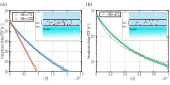
\includegraphics[width=0.99\textwidth]{03_Figure_3_2D_gaussian_with_single}%
\caption{\textit{\textbf{Two-dimensional molecular diffusion probed with a Gaussian beam.} 
(a) Interphoton delay probability density function (PDF) for the case 
of high concentrations of molecules, with an average
number of molecules $\langle N \rangle=7.5$ or $120$ in the detection area 
$A=\pi\sigma^2$ (corresponding to approximately $14$ and $225$ molecules 
per $\upmu\mbox{m}^2$, respectively). The circles are experimental values 
while the dashed lines are fits with the model from Eqn. (\ref{eq:gaussian2d}). 
(b) Interphoton delay probability density function for the case of a low concentration
of molecules, $\langle N \rangle=0.5$ (approximately $0.9$ molecules per $\upmu\mbox{m}^2$). 
In this case we find clear deviations from our model of slow diffusion, possibly indicating averaging of number fluctuations by diffusion, and a more exponential-like decay. The insets show a scheme of the experimental configuration of the lipid bi-layer on the glass surface with the typical dimensions involved (not to scale).
\label{fg:gaussian2d}}}
\end{figure}

We performed the experiment for high and low concentrations 
of molecules in the lipid bilayer and fitted 
the experimental interphoton curves with $p_{G}(\tau)$ from 
Eqn. (\ref{eq:gaussian2d}) using the experimental value for the beam 
waist, $\sigma=292$ nm. Figure \ref{fg:gaussian2d} shows the experimentally 
obtained interphoton delay probability density function for high (a) and 
low (b) concentrations along with the corresponding fits using our theoretical result. 
We note that the higher the concentration, the more the delay distribution 
resembles a single exponential. Indeed, a single exponential is expected in 
the limit of extremely high concentrations, where fluctuations $\Delta N$ 
of the number of molecules $\langle N \rangle$ in the Gaussian area become 
negligible, leading to a constant detected intensity and therefore to a single-exponential 
interphoton delay distribution.

A closer look at the curves in Fig. \ref{fg:gaussian2d} 
reveals that the case of high concentration is well captured 
with our model while the low concentration case is not. This is a direct 
consequence of the main approximation in our model, that largely neglects the 
effect of diffusion. Another phenomenon we have ignored is photobleaching of 
the molecules in the laser beam. These deviations from our model could thus be
studied through the interphoton delay distribution. 


\section{Interphoton delay distribution with fluorescence enhancement\label{sec:model_enha}}

We now turn to the case of plasmonic enhancement by an individual
nanoparticle. The spatial distribution of fluorescence enhancement by 
a plasmonic structure is complex and depends on many parameters. For 
simplicity's sake, we model this distribution as a spherically symmetric 
profile around a spherical nanoparticle. The fluorescence intensity 
profile is taken as the sum of a Gaussian confocal volume similar to 
that of the previous section, and of a near-field component modeled as 
a steeply decaying power law of radius: 
\begin{equation}
I(r) = W_0 \left[ \exp \left(-\frac{r^2}{\sigma^2} \right) + E \left(\frac{R_{NP}}{r}\right)^\alpha  \right]\,, 
\quad r \leq R_\textrm{NP}
\label{eq:enhancement_model}
\end{equation}
where $W_0$ is the unenhanced intensity, $\sigma$ the width of the Gaussian 
illumination, $E$ the maximum enhancement factor at or close to the 
particle's surface, and $R_\textrm{NP}$ the nanoparticle radius. The 
exponent $\alpha$ is a free parameter used to simulate the short-range 
variation of the near field. For pure excitation enhancement by a electrostatic 
dipole field $\alpha =6$, for combined excitation and radiative enhancements 
of an electrostatic dipole field, we would have $\alpha =12$.
We note that to recover the Gaussian case studied in the previous 
section, we need to take $R_\textrm{NP}=0$. In order to obtain 
$p(\tau)$ we insert Eqn. (\ref{eq:enhancement_model}) into Eqn.
(\ref{eq:result}) and numerically solve the integral for $R_\textrm{NP}=25$ nm. 

\begin{figure}
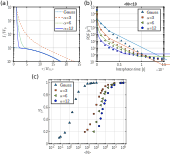
\includegraphics[width=0.95\textwidth]{04_Figure_4_enhancement_model_beta}%
\caption{\textit{\textbf{Simple model for plasmonic enhancement in two dimensions.} 
(a) Normalized radial intensity distributions for Gaussian (blue doted line), $\alpha=3$ (red dashed line),
$\alpha=6$ (green dashed line) and $\alpha=12$ (blue solid line). For all the cases the 
unenhanced intensity is $W_0=1.5\times10^4\,\mbox{cps}$ and for the enhanced case we used
$R_\textrm{NP}=25 \,\mbox{nm}$ and $E=1000$.
(b) Interphoton delay probability density function for the three cases presented in (a)
for a mean number of molecules $\langle N \rangle =10$ in the Gaussian area. The symbols present
the data from the numerical evaluation of $p(\tau)$ and the solid lines are fits with a stretched exponential. 
We intentionally reduced the density of points for display.
(c) Extracted $\beta$ from the stretched exponential fit as a function of the mean number of 
molecules in the Gaussian area. The color code is maintained throughout the whole figure. 
\label{fg:enahncement_model}}}
\end{figure}


Figure \ref{fg:enahncement_model} (a) shows the comparison 
of the spatial intensity distribution for three different 
values of the exponent $\alpha$ with the unenhanced case. 
With these intensity spatial distributions, we calculated the interphoton
delay distribution by numerically solving the integral in Eqn. (\ref{eq:result}). 
Note that the area inside the nanoparticle is not accessible 
to the molecules so the integration was carried for $r \geq R_\textrm{NP}$.
The obtained distributions are shown in Fig. \ref{fg:enahncement_model} (b) 
for the case of $\langle N \rangle=10$ molecules in the Gaussian area ($A=\pi \sigma^2$).  
Clearly the distributions with enhancement show more probability density at extremely 
short interphoton times, corresponding to the high emission rates produced by 
molecules occasionally entering the near-field area with high enhanced intensities. 
These events correspond to bright bursts in the fluorescence time trace. 
The lower the concentration of molecules, the more seldom these events will be, 
and the further away the delay distribution will be from a single exponential. 

In order to qualitatively compare the interphoton delay distributions for the 
different cases, we decided to fit them with stretched exponentials:
\begin{equation}
f(\tau) = A \exp\left[ -(\lambda \tau)^\beta\right]
\label{eq:strechted_exp}
\end{equation}
to characterize the deviation of the interphoton delay distribution from a single 
exponential. As we mentioned before, in the case of very high molecular concentration 
we expect to recover $\beta=1$, i.e. an exponential behavior, whereas large number 
fluctuations will give rise to strong deviations from single exponential and to a smaller 
stretching exponent. The empiric fit function in Eqn. (\ref{eq:strechted_exp})
works reasonably well for short times, but fails to reproduce the long-time tails of the 
delay distribution. Therefore, we focus our analysis on the short-time domain, which contains 
the most useful information about plasmonic enhancement.


We fitted the calculated probability density functions for different concentrations of molecules
ranging from a very diluted sample ($1$ molecule in the Gaussian area, $3\times10^{-3}$ 
in the near-field area) to an extremely 
high number of molecules ($10^{6}$ in the Gaussian area, $3\times10^{3}$ in the near field). 
Figure \ref{fg:enahncement_model} (c) 
shows the obtained stretching exponent $\beta$ as a function of concentration and for the Gaussian
beam and the enhanced case with three different exponents $\alpha =3$, $6$, and $12$.
In the Gaussian case we obtain an exponential behavior, 
characterized with $\beta=1$ only for $\langle N \rangle \geq 100$. This corresponds
to the situation when number fluctuations in the
detection area are negligible and thus a nearly constant detected intensity is obtained. 

To obtain a single-exponential interphoton delay distribution in the enhanced case, 
we should reach the high-density regime mentioned above, but considering the near-field area.
Since the ratio of the near-field area $A_\textrm{NF}$ (consider as the area 
that contains intensities higher than $EW_0\exp(-1)$) and the far-field area 
$A_\textrm{FF}=\pi\sigma^2$ is $\frac{A_\textrm{NF}}{A_\textrm{FF}} \sim 3\times10^{-3}$,
we roughly expect a difference of $3$ orders of magnitude in the number of molecules 
needed to reach the single-exponential limit. Indeed, this is what our
curves show, where for the enhanced case we approach $\beta=1$ around 
$\langle N \rangle=10^5$. 

From Fig. \ref{fg:enahncement_model} (c), we see that the stretching exponent steeply 
decreases with concentrations, as expected from the qualitative discussion above. 
This effect is more pronounced for a steeper decay of the fluorescence intensity 
profile, i.e., for larger values of $\alpha$. For very small concentrations, the 
stretched-exponential fit becomes poor, and the associated beta values have been 
omitted. We also note that the slope of the variation of $\beta$ with concentration 
is not very sensitive to the near-field decay characterized by $\alpha$ 
(see Fig. \ref{fg:enahncement_model} (c)). 


\section{Fluorescence time traces with enhancement by a gold nanorod \label{sec:enhancement}}

We now turn to results of an experiment with configuration similar to the one 
presented in section \ref{sec:gaussian2d}. A Gaussian beam is focused on a 
single gold nanorod immobilized on a glass substrate, and dye molecules diffuse 
in a lipid bi-layer deposited on the same substrate, similar to Ref. \cite{pradhan2016goldnanorodenhanced}. 
A fluorescence signal is produced whenever a dye molecule enters the 
diffraction-limited Gaussian beam, and an enhanced fluorescence 
signal appears if the molecule then enters either of the plasmonic hot spots 
around the tips of the gold nanorod. In order to obtain the enhancement value, 
we need to compare the detected intensity from a single-molecule enhancement event 
with the unenhanced intensity detected using the same experimental conditions, which 
was $100$ kcps\cite{pradhan2016goldnanorodenhanced}.

\begin{figure}
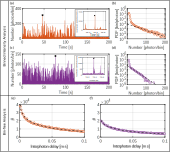
\includegraphics[width=0.95\textwidth]{05_Figure_5_enhancement_traces}%
\caption{\textit{\textbf{Single-molecule fluorescence enhancement by gold nanorods.} 
The top panel shows the typical binned-intensity plots while the bottom 
panel shows the bin-free interphoton histograms.
(a),(c) $1$ms-binned fluorescence intensity as a function 
of time for two individual nanorods. The nanorod in (a) presents
a higher enhancement factor. The black cross in the plot indicates the 
maximum recorded intensity. The insets show respective zooms around the maximum
intensity bursts.
(b),(d) Burst intensity histograms showing number of photons per $1$ms-time bin for the traces in (a) and (c), 
respectively. The dashed black lines are exponential fits to the tail of the distributions. 
(e),(f) Interphoton delay probability distributions for the experimental traces 
shown above. We also show a fit to the curves using a stretched-exponential model.
The curves in purple (orange) correspond to traces (a) and (c) respectively and this color code is maintained throughout the whole figure. 
\label{fg:GNRS}}}
\end{figure}
% left in comment what michel wrote
%- brief description of time trace (see Ref. \cite{pradhan2016goldnanorodenhanced}) with long weak bursts corresponding to far field and occasionally intense but short bursts corresponding to diffusion in the near field. For the traces shown, the selection of the highest burst(s) lead to enhancement factors of XXX.

Figure \ref{fg:GNRS} presents the TTRR experimental data obtained in 
such an experiment in different ways, for two different gold nanorods. 
In the top panel we have the bin-dependent time traces and burst histograms (binning time $1$ ms) while the lower panel
shows the ``bin-free'' interphoton delay histograms.
If we analyze the binned time traces in Fig. \ref{fg:GNRS} (a) and (c) and the insets, we observe that they
present a qualitatively similar behavior: there is a constant baseline
intensity, long weak bursts corresponding to molecules exploring the far field area and occasionally 
intense but short bursts corresponding to diffusion in the near-field area\cite{pradhan2016goldnanorodenhanced}. 
The black crosses in the time traces indicate the highest burst found in that trace, which leads to 
``cherry picking'' enhancements factors $E^{(CP)}=(4.5 \pm 1.5)$ and $E^{(CP)}=(2.3\pm 0.7)$.

%- characterization of time trace by histogram of binned data; comparison of histograms for two types of nanorods, one with weak enhancement, the other with stronger enhancement. Discuss the histograms and the decay of probability with number of photons per bin. Physical interpretation: unlikely to have strong bursts because the molecule has to come very close to the nanorod tip, probability decays as distance in 2D, square of distance in 3D.

%- Should give a power law, but experimentally resembles more an exponential cutoff. Possible reasons for that deviation: photobleaching, detector limitations, possibly role of diffusion during the measurement of the burst.

Another useful way to characterize the experimental enhancement is the histogram 
of binned intensities, as shown in Fig. \ref{fg:GNRS} 
(b) and (d). These histograms show a rapidly-decaying tail where the characteristic 
decay intensity is larger for the top nanorod, indicating stronger enhancement. The 
steep decay of these histograms can be qualitatively understood by recalling the spatial 
distribution of near-field intensity at resonance, which is
extremely high (around $300$ times the incident intensity) very close to the tips and 
decays rapidly with distance to the tips. 
Therefore, there is a low probability for a diffusing molecule to reach this small area. 
For small distances, this probability density goes linearly with distance 
in the bi-dimensional case, and as the squared distance in three-dimensional case. 

We analyzed the intensity distribution around a rod ($25\times47$ nm$^2$), calculated 
from a discrete-dipole approximation \cite{khatua2014resonant}. In the 2D case, we found an 
approximate power law distribution with exponent $1.37$. However, the tail of the 
experimental distribution is exponential, as can be seen in Fig. \ref{fg:GNRS} (b) and  Fig. (d).
There are several possible sources for such a discrepancy, such as the effect of photobleaching,
the dead time of the detectors, and possibly the role of diffusion during the burst.
Confirming the role of each of these effects would require full numerical calculations, with 
an accurate description of these effects. However, this is a complex and computationally 
extensive problem that is out of the scope of this paper.

%- Whatever the reason for this deviation, we may estimate the maximum enhancement through the histogram. Notice that stronger enhancement corresponds to a broader histogram, with cutoff for larger number of photons. If we model the histogram decay as a single exponential $P(N)=\exp(-N/N_0)$, we can estimate the maximum number of photons in the strongest burst as $N_0 \ln(M)$, where $M$ is the total number of attempts and is proportional to the duration of the trace. For a typical value of M=$10,000$, we find 9.2 $N_0$ (check this with the ratio of time trace to burst duration...).

Regardless of the reason for this deviation, we may empirically estimate
the maximum enhancement through the histogram. Note that stronger enhancement 
corresponds to a broader histogram, with cutoff for larger photon number.
If we model the tail of the normalized histogram decay as a single exponential $P(N)=M\exp(-N/N_0)$, 
we can estimate the maximum number of photons in the strongest burst by solving 
$P(N_c)=\varepsilon$ with $\varepsilon=1/N_{\mbox{bins}}$, where $N_{\mbox{bins}}$ is 
the total number of bins in the time trace, here about $10^6$. This estimate roughly 
corresponds to a probability equal to unity of observing such an intense burst in the 
time trace. We thus obtain $N_c = N_0 \ln(M/\varepsilon)$. For a typical value of 
$M\sim\times10^{-3}$, we find $6.9 N_0$. With this method we obtain $E^{(H)}=(4.9 \pm 0.2)$ 
and $E^{(H)}=(2.40 \pm 0.05)$ for the plotted data in Fig. \ref{fg:GNRS} (b) and (d).

%- We can also estimate the enhancement factor from the maximal intensity read from the histogram of delays between consecutive photons. These histograms are shown for two rods in Fig XXX. Deviations from single-exponentials are clearly seen. To characterize them, we fit the histograms with a stretched exponential of time $p(\tau)=A \exp(-(w\tau)^\beta)$, as this fit involved only three parameters, against four for a bi-exponential decay. The maximum intensity is deduced from the slope of the histogram at the shorter possible time and provides another estimate of the enhancement factor based on a statistical quantity. Fig XXX shows that larger enhancements correspond to a larger deviation of the histogram from a single exponential, and to a larger slope at the smallest bin time of the histogram. 

We can also estimate the enhancement factor from the interphoton delay histograms. These histograms are shown for the same
two nanorods in Fig. \ref{fg:GNRS} (e) and (f). 
Deviations from single-exponentials are clearly seen. To characterize them, we fit the histograms 
with a stretched exponential of time (see Eqn. (\ref{eq:strechted_exp})), which involves only 
three parameters, against four for a bi-exponential decay. The maximum enhanced intensity is deduced from 
the slope of the histogram at the shorter measured interphoton time ($200$ns) and provides another estimate of the 
enhancement factor based on a statistical quantity. Figures \ref{fg:GNRS} (e) and (f) 
show that larger enhancements correspond to a larger deviation of the histogram from a 
single exponential, and to a larger slope at the smallest bin time of the histogram. With 
this procedure, we obtained an enhancement value of $E^{(I)}=(4.3 \pm 0.2)$ and 
$E^{(I)}=(2.0\pm 0.1)$ for the presented nanorods.

%\subsection{Comparison of the estimates of enhancement factors by the 3 methods}

We now compare the maximum intensities and the associated enhancement factors obtained 
for five different nanorods, for the whole $200$ s-long time trace, and after splitting each trace into 5 sub-traces 
of $40$ s each. Figure \ref{fg:en_cor} shows the example of the binned time trace (a),
burst histogram (b) and the interphoton delay histogram (c) for the whole trace and for each sub-trace. 

The associated results for the different methods are correlated in Fig. \ref{fg:en_cor} (c) and (d).
The different symbols correspond to different nanorods and the colors refer to the different sub-traces for each rod. 
In Fig. \ref{fg:en_cor} (d) we observe an excellent correlation between the cherry-picking method and the
statistical method based on the burst intensity histograms. Note that the same symbols are clustered together,
showing that the enhancement factor obtained using different sub-traces with both methods lead to similar results.
We also correlated the results from the interphoton delay distribution with the burst intensity histograms in 
Fig. \ref{fg:en_cor} (e), where a satisfactory correlation is found and the obtained enhancement factors
are consistent with both other methods. However, the enhancement factors deduced from interphoton delay distributions present more dispersion than the other two. 

   

\begin{figure}
\includegraphics[width=0.99\textwidth]{06_Figure_6_enhancement_correlation}%
\caption{\textit{\textbf{Comparison of the enhancement factors obtained with different methods.} 
(a) Binned time traces split into five different sub-traces of $40$ s each (binning time $100$ $\upmu$s). 
The crosses show the maximum number of counts per bin obtained in each sub-trace, 
used to calculate the ``cherry-picking'' enhancement factor $E^{(CP)}$. At the top we show the 
length of the sub-traces and assign a number for reference.
(b) Normalized burst histogram in number of photons per bin obtained for each of the sub-traces presented in (a).  
We also show in dashed lines the exponential fits to the tail of the probability density. The burst histogram for the total trace is plotted as well.
(c) Interphoton delay distributions for the sub-traces and the total trace with their stretched-exponential fits. 
(d) and (e) show scatter plots of enhancement factors $E^{(CP)}$, $E^{(H)}$, $E^{(I)}$ deduced by the three methods. The different
symbols correspond to different nanorods and the colors refer to the sub-traces used to obtain the enhancement factor.
In black we show the results for the total trace. 
(d) Correlation between $E^{(CP)}$ from cherry picking and $E^{(H)}$ from burst histogram, showing an excellent correlation with slope equal to unity (dashed black line).
(e) Correlation between $E^{(I)}$ from interphoton delay histograms and $E^{(H)}$ (the dotted line is a linear fit with
slope $1$). Here, we observe more dispersion of the data.
}
\label{fg:en_cor}}
\end{figure}

%
%Fig(XXX) confirms that the three measures of the enhancement factor are consistent with one another. Check that more spread from cherry-picking? Has to be written once the results are available...

Figure \ref{fg:en_cor} confirms that the estimates of the enhancement factor deduced by three very different methods (time trace, burst histogram, interphoton delays) are similar in value and consistent with one another. The values deduced from the cherry-picking procedure are surprisingly stable and reliable. They agree well with extrapolations of burst histograms fitted with a single-exponential function, although the justification for this analytical form is still missing. Unexpectedly, the enhancement factor deduced from the interphoton histogram appears to be the most sensitive to statistical fluctuations. This can be a consequence of fitting with a stretched exponential, which is an approximation. However, this method has the unique advantage that it can be applied to the experimental data directly, without any need for binning or other arbitrary parameters.


\section{Conclusions}

In this paper we characterized single-molecule fluorescence traces 
obtained with a time-tagged time-resolved setup in a variety of 
experimental conditions with the \textit{interphoton
delay distribution}. This avoids the introduction of an arbitrary binning time. 

We presented a theoretical treatment for the case of nearly static, slowly diffusing molecules that
relates the interphoton delay distribution to the spatial intensity 
distribution explored by the molecules. With this model, we could reproduce the simple case of 
switching between two states with different intensities. We also explored the problem of molecules diffusing in two dimensions in a Gaussian beam. Our nearly static model works well at high concentrations, but shows deviations at lower concentrations, which may arise from diffusion or from other experimental deviations from the model.

Furthermore, we used the interphoton delay distribution to measure the 
fluorescence enhancement factor by individual gold nanorods. For our experimental traces with moderate enhancements, we obtained
enhancement factors that are consistent with the accepted methods in the 
community with the advantage of avoiding the introduction of any arbitrary
parameter that may influence the results. 
In the future, we plan to perform similar comparisons for the very 
large enhancement factors obtained with weakly emitting dyes.
%=========== Supporting info ========
% \newpage
% \section{Supporting Info}
\graphicspath{{./chapters/c3_binfree/si_figure/}}

\section*{Transient Binding sample preparation}


\section*{Binned time traces dependence with bin time}



\section*{Lipid bilayer sample preparation}



\section*{2D Numerical simulations}

The current program is organized in only one script, simualtion2d.m and contains several subroutines. It also uses the program generate\_simulation\_parameters.m to set all the needed parameters for the simulation. These are divided in two sets, the physical parameters and the simulation parameters. 
The former set of parameters corresponds to the experimentally relevant variables while the latter corresponds to the extra parameters needed to run the simulation and are not related to the experimental conditions but need to be selected to run the simulation. 
The output of the program is a structure that has contains the unbinned time traces, binned time traces and interphoton histograms. The physical inputs are the following: concentration of molecules $C$, intensity distribution of the incoming beam $I(\ve{r})$ and dark counts of the detector $Dc$. 
For a complete list of the simulation parameters, refer to the appendix \ref{ap:sim_param}.

The calculation consists of several steps that will be summarized in the following. 
The spatial intensity distribution input has to be a matrix $M$ with the spatial intensity distribution of the incoming beam $I(\ve{r})$ (in cps). 
The first step is done by the subroutine \texttt{calculate\_times} to simulate the absolute arrival photon times for each intensity value of the matrix 
\footnote{This can be improved in speed by not calculating the repeated intensity values more than one time and by saving the output structure in a file and loading it later instead of recalculating it.} 
within the time of the experiment, $T_{\mbox{Max}}$. This traces correspond to a single molecule placed in each pixel of the intensity matrix.
To generate the correct exponential distribution for a given intensity $I$, I use the fact that the interphoton times should follow an exponential distribution:
\begin{equation}
\Delta t_{i} = -\frac{\log\left(\zeta_i \right)}{I} \, ,
\label{eq:interphoton_simulation}
\end{equation}
where $\Delta t_{i}$ ($i=0,...,N$) represents the time between successive photons detection and $\zeta_i$ is a random number in the interval $(0,1)$. 
This way of generating the interphoton times ensures the required exponential distribution. Then by performing the cumulative sum over the interphoton times the absolute arrival times of the simulated stream of photons can be calculated for each intensity value in the input intensity matrix $M$. This data is contained in a structure named \texttt{abs\_times}. 

The next step is to calculate the number of molecules present in the simulation volume  $V_{sim}$. For a given concentration, the number of molecules contributing to the simulation is random variable that follows Poisson distribution with a mean value $\left<N_{molecules}\right> = C V_{sim}$. Since our calculation is based on the calculation of the interphoton arrival time for a fixed number of molecules $N_{molecules}$ in the simulation volume, we calculate the number of molecules needed to contain 99\% of the cases. Then, for each $N_{molecules}$ we generate the interphoton histogram as follows. We generate random positions for all the available molecules in the simulation volume and we retrieve the corresponding absolute photon arrival times from the variable abs\_times. We concatenate all this arrival time and also include extra photon detections generated by the dark counts of the detector. The mean number of dark photons in the simulation time is $Dc T_{\mbox{max}}$ and follows a poisson distribution. We use a poissonian number generator to simulate the number of detected photons in each run and then distribute them uniformly in the time trace. All this concatenated absolute photon detection times are then sorted and saved in a vector $t$. Then the histogram of the interphoton times for this vector is computed, using pre-fixed bins (with a certain number of points $Hist_{\mbox{Npts}}$) . The normalized (to the total counts) histogram is stored into the first component of a matrix of histogram counts $H$. Then we repeat this procedure $N_{\mbox{config}}$ time, using each time a new set of random positions for all the molecules, creating the matrix of dimensions $Hist_{\mbox{Npts}} \times N_{\mbox{config}}$. Then we average the normalized histograms corresponding to different spatial configurations, contained in $H$ to obtain a single histogram corresponding for a single number of molecules in the simulation volume. The final step is to perform a weighted average of the histograms for each number of molecules contributing to the simulation for a fixed concentration using the corresponding poissonian weight.



\section*{Slow diffusion case}

We simulated the case of a molecule 


\section*{Simulation Parameters\label{ap:sim_param}}

\section*{code validation\label{ap:code}}

In order to validate the simulation code we tested the results with a simple beam shape that provides an analytical solution. 
We work in two dimensions just for simplicity with a rectangular beam shape with constant intensity and zero intensity outside, described mathematically as:
\begin{equation}
I(x,y) = I_0\theta(|x-\frac{x_0}{2}|)\theta(|y-\frac{y_0}{2}|)\, ,
\label{eq:theta_intensity}
\end{equation}
with $I_0$ the maximum intensity and $x_0,y_0$ the size in lateral directions and $\theta(\zeta)$ the step function. Thus, the illuminated area has a volume of $V_0=x_0y_0$. 
For such a beam shape the interphoton probability distribution can be obtained by simple integration of equation \ref{eq:result} replacing the beam shape $I(\ve{r})$ with equation \ref{eq:theta_intensity}, obtaining
\begin{equation}
p(\tau) = I_0 C V_0 \exp[-\tau I_0-C V_0(1-\exp(-\tau I_0))]\,.
\label{eq:theta_interphoton_distribution}
\end{equation}

Figure \ref{fg:square_beam}(a) shows an example in a particular case when the dimensions are the same for the two directions and \ref{fg:square_beam}(b) shows plots for the analytical solution for different intensities and concentrations.




 \begin{figure}
 \centering
 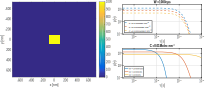
\includegraphics[width=\textwidth]{square_illumination}%
 \caption{\textbf{Simple illumination profile that provides an analytical solution to test the simulation code} 
(a) Colormap plot of the square-shaped beam we use for validating the code. We used $x_0=y_0=182$ nm and $I_0=1000$ cps.
(b)Analytical plots of the interphoton probability distribution for different intensities and concentrations. 
\label{fg:square_beam}}
 \end{figure}


%\figdouble{square_illumination}{square_illumination_analytical}{fg:square_beam}{Simple illumination profile that provides an analytical solution to test the simulation code}{ \figa Colormap plot of the square-shaped beam we use for validating the code. We used $x_0=y_0=182$ nm and $I_0=1000$ cps. \figb }


In order to test the code we performed simulations using this illumination distribution and compared it with the analytical result. We started with a fixed superficial concentration  C=$2 \times 10^{-4}$ molecules nm$^2$ to have a relative fast run and we changed the different parameters of the simulation, such as the number of spatial configurations to average and the total simulation time $T_{\mbox{max}}$. The comparison with the analytical curves can be seen in figure \ref{fg:sim_test}. In both cases the simulation agrees well with the analytical result and for longer simulation time or higher number of configurations, the error becomes smaller.


 \begin{figure}
 \centering
 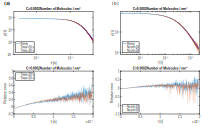
\includegraphics[width=\textwidth]{Theta_results}%
 \caption{\textbf{Test of simulation parameters and code validation} 
(a) Different total simulation times. Top: simulated and analytical curves. Bottom: relative error in the simulation.
(b) Different number of averaged spatial configurations. Top: simulated and analytical curves for different total simulation times $T_{\mbox{max}}$. Bottom: relative error in the simulation.
\label{fg:Theta_results}}
 \end{figure}


The next step was to test the simulation for different physical parameters such as the concentration of molecules and the intensity in the beam. The results for three different concentrations and intensities can be found in figure \ref{fg:phy_test}. The results again agree with the analytical curves and it can be noted that the larger the number of photons generated in the simulation the better correspondence with the analytical result.


 \begin{figure}
 \centering
 \includegraphics[width=\textwidth]{Theta_physical_test}%
 \caption{\textbf{Test of physical parameters and code validation} 
(a) Different concentrations. Top: simulated and analytical curves. Bottom: relative error in the simulation.
(b) Different intensities. Top: simulated and analytical curves. Bottom: relative error in the simulation.
\label{fg:Theta_physical_test}}
 \end{figure}
% \references{chapters/c3_binfree/biblio}
%  \chapter{DNA transient binding on a gold nanorod}
\label{chapter:transient}
\graphicspath{{./chapters/c5_transient_binding/figures/}}

%============================== MAIN =======================================
\begin{abstract}
  Fluorescence enhancement by plasmonic nanostructures enables the detection of dyes with low quantum yield and improves the yield of quantum solid-state light sources.
  Here we demonstrate a DNA-based transient binding method to repeatedly and reproducibly study many single molecules by fluorescence enhancement on a single nanorod at the same spot on its tip.
  Heterogeneity of excitation and emission enhancements is avoided by looking at the same nanorod and the same binding site repeatedly.
  Bleaching of the plasmonic enhanced single molecules is no longer a problem as the bleached molecules are replaced by new ones.
  We characterize the distribution of enhancement factors and binding times. We investigate the fluctuations of the enhanced signal and the long-term stability of the binding sites.
\end{abstract}

\newpage
\section{Introduction}
Plasmonic nano-structures confine light to much smaller spatial dimensions than the optical diffraction limit. They enable detection of single molecules even at micromolar or millimolar concentrations, which is otherwise extremely challenging in conventional microscopy.\cite{levene2003zeromode,punj2013a,schuller2010plasmonics}
Optical nano-antennas strongly interact with quantum emitters, modifying their excitation and emission rates, and opening new non-radiative dissipation channels.
For emitters placed at the right position, plasmonic antennas can enhance their fluorescence by two to four orders of magnitude, enabling the detection of dyes with poor quantum yields.\cite{lakowicz2005radiative,anger2006enhancement,kinkhabwala2009large,acuna2012fluorescence,yuan2013thousandfold,khatua2014resonant}
The high electric field near the antenna leads to excitation enhancement while the high local density of optical states enhances the emission rates of the emitters, often leading to improvement in the brightness.
For emitters placed close to the metal surface, the nano-structure acts as an energy sink, quenching the fluorescence.\cite{seelig2007nanoparticleinduced,muskens2007strong,acuna2012distance,matsuzaki2017strong}
However, emission enhancement and quenching are highly dependent on the position of the dye with respect to the plasmonic structures. Therefore, fluorescence enhancement in the vicinity of nanoantennas is strongly inhomogeneous, because of the inhomogeneous electric field near the plasmonic structures, and because the position of the emitters cannot be controlled accurately. 


Different approaches to study single molecules by fluorescence enhancement involve free diffusion, non-specific sticking or immobilization of the emitters around the nanostructures. All of those approaches lead to random positioning of the emitters around the antenna.\cite{pradhan2016goldnanorodenhanced,yuan2013thousandfold,zhang2017gold}
This results in inhomogeneous excitation and emission of the fluorophores.
Uniform excitation and a better understanding of the photophysics of the fluorescent probes are necessary to fully understand the activity of biological or chemical systems as the light itself can perturb the system under study.
For instance, recently we found that the different excitation rates in the near field of a gold nanorod led to variations in midpoint potential of a redox indicator (methylene blue). The origin of this change was not clear as we could not precisely control the position of the dye.\cite{zhang2017gold}
The diffusion or immobilization methods also pose a limit to the observation time of the single molecules.
Diffusion times in the near field are often faster (\SIrange{1}{1000}{\us}) than the biomolecular processes (\SI{>1}{\ms}) making it difficult to study the slower process.
Whereas molecules can be immobilized almost indefinitely by chemical binding, bleaching limits their observation time. With immobilization by chemical binding, the number of single molecules that can be studied is thus limited to one per nano-antenna.


Here, we propose a transient binding method, by which fresh single dye molecules can be transiently immobilized on the same plasmonic hot spots. Nucleic acids, in particular DNA, offer highly predictable base pairing and binding energy, providing a simple and elegant mechanism for transient binding. Transient binding of short DNA strands has been applied in a super-resolution imaging technique called DNA-PAINT.\cite{jungmann2010singlemolecule,lin2012submicrometre,schnitzbauer2017superresolution}
The necessary blinking required for super resolution is generated by the transient binding of the short dye-labeled DNA ('imager') to its complementary target ('docking') strands on the structure in vitro or in vivo.
The chemistry and kinetics of single-strand DNA (ssDNA) binding are well understood at single-molecule level and widely available, thanks to the rapid development of DNA-PAINT and DNA-based biosensors.\cite{sassolas2008dna,jungmann2010singlemolecule}
The binding time of the imager strand to the docking strand can be tuned by the electrolyte concentration, the number of base pairs, the temperature, while the distance of the molecule to the antenna can be controlled by the number of base pairs, with a resolution of \SI{0.33}{\nm} per base pair.
Moreover, as DNA has a persistence length of \SI{\sim50}{\nm}, it acts as a rigid tether, thereby stabilizing the distance between the molecule and the plasmonic nanostructure.\cite{manning2006the}


In the current study, we chose gold nanorods as the plasmonic nanoantenna because of their simple structure, the high tunability of their surface plasmon resonance (SPR) and the accessibility of their near field to bigger molecules such as proteins and other biomolecules.
The nanorod can enhance the optical excitation intensity by two to three orders of magnitude when irradiated with a resonant laser.
The fluorescence enhancement relies on the overlap of the spectrum of the dye with the SPR of the rod and the laser excitation.
The optimum distance for enhancement is \SIrange{3}{5}{\nm}; closer to the rod, fluorescence quenching will dominate; too far away from the rod, the excitation enhancement will fade.\cite{khatua2014resonant}
With a linker of 10 base pairs, the distance of the dye to the surface is \SIrange{3.5}{4}{\nm}, provided the dye is at the further end of the imager strand.
By adjusting the concentration ratio of docking strands to passivating ligands, we can tune the average number of docking strands per rod, down to less than one per rod. The binding of the docking strand being a random process, the probability of having the docking strand on one of the tips of the rod will scale as the ratio of near-field area to total rod area.
In the present work, we wish to characterize the enhancement factors, the binding times, and the flexibility of the docking strand attached to the nanorod. Moreover, we show that a single gold nanorod with the right binding site is enough to study fluorescent enhancement with a statistically significant number of single molecules.


%====================EXPERIMENTAL SECTION=======================
\section{Methods}
\paragraph*{Materials.} Ethanol (\SI{99.8}{\percent}), methanol (\SI{99.8}{\percent}), 3-Mercaptopropyl) trimethoxysilane (MPTS, \SI{95}{\percent}), cysteamine (\SI{98}{\percent}), thioglycolic acid (\SI{99}{\percent}), Potassium chloride (\ce(KCl)), 4-(2-Hydroxyethyl) piperazine-1-ethanesulfonic acid (HEPES, \SI{99.5}{\percent}), Bovine serum albumin (BSA, \SI{96}{\percent}), Tris(2-carboxyethyl) phosphine hydrochloride (TCEP, \SI{98}{\percent}) were purchased from Sigma-Aldrich; 
Magnesium chloride (\ce{MgCl2}), Hydrogen peroxide (\ce{H2O2}, \SI{30}{\percent}), Sodium acetate (\ce{CH3COONa}, \SI{99}{\percent}), Potassium dihydrogenphosphate (\ce{KH2PO4}), disodium hydrogenphosphate (\ce{Na2HPO4}) from Merck;
Ammonium hydroxide (\ce{NH4OH}, \SI{30}{\percent}), Hydrochloric acid (\ce{HCl}, \SI{37}{\percent}) from Acros Organics;
succinimidyl 4-(p-maleimido- phenyl) butyrate (SMPB) from ThermoFisher.
Phosphate buffered saline (PBS) pH 7.4 contained \SI{137}{\mM} \ce{NaCl}, \SI{2.7}{\mM} \ce{KCl}, \SI{10}{\mM} \ce{Na2HPO4} and \SI{1.8}{\mM} \ce{KH2PO4}.
HEPES pH 7 buffer contain \SI{20}{\mM} HEPES. Acetate buffer pH 4 was prepared from \SI{164}{\mM} \ce{CH3COOH} and \SI{36}{\mM} \ce{CH3COONa}.


\paragraph*{Oligonucleotides.} The following DNA oligonucleotides were purchased from Integrated DNA Technologies:
\begin{itemize}
	\item DTPA-5'-ATA CAT CTA GAA ATT-3' (docking strand)
	\item -----3'-TAT GTA GAT C-Cy5-5' (imager strand)
\end{itemize}
Here DTPA represents a hexacyclic group with a dithiol that is used to strongly bind to gold, Cy5 denotes a red Cyanine dye, and A, T, C, G denote the DNA bases. Ten bases of docking strand are complementary to ten bases in the imager strand. The chemical structures and the binding scheme are shown in Figure S\ref{SIfig:AuNR-SS_bonding}.


\paragraph*{Silanization of glass surface.} Glass coverslips (Menzel-Glaser, \SI[product-units=repeat]{22x40}{\mm}, no. 1 thickness) were cleaned and activated for silanization before further functionalization.
The coverslips were sonicated in water (\SI{15}{\minute}) and ethanol (\SI{15}{\minute}). 
Then they were heated  at \SI{70}{\celsius} in a bath containing \ce{H2O}/\ce{NH4OH}/\ce{H2O2}(5:1:1) to remove organic impurities from the surface.
This step made the surface hydrophilic indicating the abundance of hydroxyl functionalities on the surface.
The cover slips were rinsed thoroughly in water and stored in ethanol for further use.
To activate the surface, the coverslips were flamed and treated for 30~min in a Teflon incubator with a \SI{1}{\percent} solution of (3-Mercaptopropyl)trimethoxysilane in methanol containing \SI{5}{\percent} glacial acetic acid.
Then the glass slides were rinsed and baked in an oven at \SI{65}{\celsius} for \SI{3}{\hour}.
This results in binding of the silane groups to the active hydroxyl groups and creates a thiol surface that can be used for conjugation with gold nanorods and for passivation of the substrate surface.


\paragraph*{Gold nanorod functionalization.} Gold nanorods (AuNRs) were synthesized using previously published seed-mediated growth in cetyl trimethyl ammonium bromide (CTAB). \cite{nikoobakht2003preparation}
The longitudinal surface plasmon of the AuNRs was \SI{640}{\nm} as obtained from the UV-vis spectrum, and their average dimensions were $\SI{90}{\nm}\times\SI{45}{\nm}$ as obtained from scanning electron microscopy images.
Excess of CTAB was removed by centrifugation and resuspension in milliQ water.
A thiolated coverslip was mounted in a homemade flow cell.
The AuNR solution was sonicated and immediately incubated in the flow cell for 10~min and then washed off with PBS buffer.
This resulted in around 10 isolated single gold nanorods per \SI{100}{\um\squared} area on the substrate.
A mixture of \SI{1}{\nM} thiolated docking strands and \SI{10}{\uM} methoxy-poly(ethylene glycol)-thiol (mPEG7-SH, MW 350) in pH 4 buffer was incubated overnight.
mPEG7-SH was used as the passivating ligand and allowed us to control the average number of docking strands on the nanorod.
The ratio between docking strands and passivating molecules was varied to get the desired number of docking strands at the tip of the nanorod.
The length and chemical nature of the passivating ligands were varied to test the flexibility of the docking strand.
Unless mentioned otherwise, the passivating ligand was mPEG.


\paragraph*{Surface passivation.} To prevent the unspecific sticking of imager strands to the surface, the rest of the glass surface was functionalized with bovine serum albumin (BSA).
This was achieved by incubating the coverslips with \SI{1}{mM} succinimidyl 4-(p-maleimidophenyl) butyrate (SMPB), \SI{20}{\uM} BSA and \SI{1}{mM} Tris(2-carboxyethyl)phosphine hydrochloride (TCEP) in HEPES pH 7 for \SI{1}{\hour}.
The succinimidyl group of SMPB binds to the BSA while its maleimide group binds to the thiol on the substrate. 
The unreacted chemicals were washed off with PBS pH 7 buffer.


\paragraph*{Imaging and time trace recording.} All the measurements were performed in a home-built confocal microscope that was equipped for Time Correlated Single Photon Counting (TCSPC).
Light from a pulsed picosecond diode laser (Power Technology, Little Rock, AR, USA) with a repetition rate of \SI{40}{\MHz} and a wavelength of \SI{635}{\nm} was passed through a narrow-band clean-up filter (Semrock LD01-640/8-25), then coupled into a single-mode optical fiber.
The output was collimated using a telescope system and reflected by a polychroic mirror (z488/633rpc) onto the back aperture of a high-numerical-aperture oil immersion objective (NA=1.4, Olympus UPLSApo 100x) and then focused to a diffraction-limited spot (\SI{300}{\nm}) on the surface of the coverslips.
An intensity of \SI[per-mode=repeated-symbol]{100}{\watt\per\cm\squared} was used to image the fluorescent objects on the surface.
Epi-fluorescence from the focal volume was collected through the same objective and focused on a pinhole for spatial filtering, and then passed through an emission filter (z488/635m "dual"-band emission filter, Chroma) to get rid of scattered laser light.
Finally, the fluorescence light was focused onto the active area of an avalanche photodiode (SPCM AQRH-15, Perkin Elmer Inc., USA).
The data was recorded by PicoHarp 300 (PicoQuant GmbH, Berlin, Germany) in time-tagged-time-resolved (t3r) mode which stores both arrival time and micro-time (time after laser excitation) of each photon.


Fluorescence images of the surface of the substrate were acquired by scanning a \SI[product-units=power]{10x10}{\um} area with a step size of \SI{50}{\nm} and a dwell time of \SI{1}{\ms}.
As the nanorods have very short photoluminescence lifetimes (shorter than the instrument response function IRF), they are easy to distinguish from the background of Cy-5 dye, with much longer fluorescence lifetime (see Figure S\ref{SIfig:trans_int_lt}).
The locations of the nanorods were saved and time traces were recorded for \SI{100}{\s} by parking the laser on the nanorods.
The laser intensity was \SI[per-mode=repeated-symbol]{10}{\watt\per\cm\squared}, 10 times smaller than the one used for imaging.
The nanorods with the desired number of transient-binding sites (inferred from the number of intensity levels) and fluorescence enhancement factor were selected for further measurements at different experimental conditions and durations.
%=======scheme========
\begin{figure}
	\centering
	\includegraphics[width=\linewidth]{scheme}
	\caption{\textbf{Transient binding schematic:}(left) Nanorods are immobilized on a thiolated glass surface and functionalized with docking strands and passivating ligands (mPEG7-SH).
	The coverslip surface is passivated with BSA to prevent non-specific sticking of imager strands to the glass.
	The imager-Cy5 strands in the solution  are shown with a gray dot on one end representing unenhanced fluorescence.
	One of the imager is bound to the docking strand at the tip of the nanorod and is shown with a bright red spot representing plasmon-enhanced fluorescence.
	(right) Reversible transient binding on the docking sites on a nanorod. The docking strand at the tip of the nanorod gives rise to enhancement while the one on the side of the rod exhibits no enhancement.}
  	\label{sch_trans:setup}
\end{figure}


\section{Results and discussion}
%========one vs many binding sites========
\paragraph{Number of binding sites.} The average number of docking strands on a gold nanorod is controlled simply by changing the concentration ratio between the docking DNA and mPEG7-SH.
Figure \ref{fig:timetrace1vsmany}(a) shows the time trace of transient binding on a gold nanorod with the ratio between docking and passivating strand maintained at 1:2000 and Figure \ref{fig:timetrace1vsmany}(c) at a ratio of 1:10000.
The concentration of imager strand was \SI{100}{\nM} with \SI{500}{\mM} \ce{NaCl} in PBS pH 7.4 buffer.
At ratio 1:2000, intensity bursts with different heights were observed and $5$ different peak heights can be distinguished from the intensity histogram with the maximum count rate at \SI{120}{ kcps} indicating an enhancement factor of $\sim60$ taking the count rate of un-enhanced imager as \SI{2} { kcps} (see Supporting Information, Fig S\ref{SIfig:timetrace_only_Cy5}).
The different peak heights are shown by the dashed lines and the numberings are done in increasing order of count rates.
The highest intensity shown by the arrow has two step-wise intensity changes resulting from two binding and unbinding events occurring during the same burst.
At ratio 1:10000, two intensity levels can be clearly distinguished both from the time trace and intensity histogram with the maximum enhancement factor of $\sim10$.
In all measurements, we adapted the laser power to the bursts to be detected, down to a factor of two in enhancement.
\begin{figure}[ht]
	\centering
	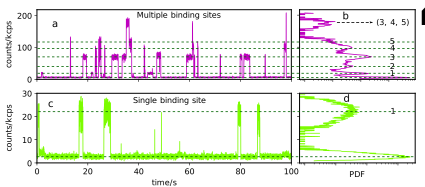
\includegraphics[width=\textwidth]{timetrace1vsmany}%width=\textwidth
	\caption{Time traces of transient binding of \SI{100}{\nM} imager with the docking sites on a gold nanorod with ratios between docking and passivating ligands of 1:2000 (a) and of 1:10000(c).
	The corresponding intensity histograms are shown on the right (b, d).
	The dashed lines connect the peaks in the histogram to the intensity levels in the time trace and the numberings are done in increasing order of the intensities.
	The arrow represents the combination of any two arbitrary levels from 1 to 5. 
	}
  	\label{fig:timetrace1vsmany}
\end{figure}


The gold nanorods were completely functionalized with mPEG7-SH and docking strands by overnight incubation.
Hinterwirth et al. showed that the coverage of \ce{PEG_7} on gold nanoparticles is \SI{4.29}{\per\nm\squared} and the packing density is mostly dependent on the steric hindrance rather than the chemical nature of the ligand.\cite{hinterwirth2013quantifying}
Therefore, a nanorod with dimensions \SI[product-units=repeat]{90x45}{\nm} should bind $5.5\times10^4$ chains, assuming similar reactivity of the passivating ligands and the docking strands.
At ratio 1:2000 between docking and mPEG7, out of ${\sim}27$ docking strands on the gold nanorod, ${\sim}5$ docking sites are observed through the fluorescence enhancement of imager strands by the gold nanorod.
Similarly, at 1:10000 ratio between docking and mPEG7 strands, ${\sim}1$ docking site is observed out of ${\sim}5$ docking strands on the nanorod.
The ratiometric study at two concentrations shows that \SI{20}{\percent} of the attached docking strands show fluorescence enhancement.
Assuming uniform distribution of the docking strands on the nanorod surface, the effective area on the nanorod for fluorescence enhancement can be calculated as \SI{20}{\percent} of its total area. We can thus estimate that the hot spots leading to a fluorescence enhancement larger than 2 times present an area of about \SI{1500}{\nm\squared} around each tip. This effective area will depend on the spectral overlap of the SPR of the rod with the dye spectra and laser, on the quantum yield of the dye, and on the distance of the dye to the surface of the rod.


One of the motivations for the present study is to observe the enhancement over and over again for the same binding site.
Figure S\ref{SIfig:bleaching_free_longtrace} shows transient binding on three different gold nanorods with different enhancement factors.
The two peaks in the intensity histogram of each rod and the absence of multi-step intensity bursts indicate that there is only one observable docking strand.
The narrow distribution of binding and unbinding times of imager strands on each particular nanorod over a time scale of \SI{1000}{\s} indicates that there is little variation in the DNA binding site over time.
However, the frequency of binding and unbinding varied from nanorod to nanorod, even for rods with a similar enhancement factor (Fig S\ref{SIfig:bleaching_free_longtrace}A, C).
This variation can be attributed to the different local environments in the PEG brush around each individual binding site, which can hinder the approach and binding of the imager strand to the docking strand.
For very long experiments (\SI{\sim1}{\hour}), we observed that the intensity bursts may completely disappear (Fig. S\ref{SIfig:dissociation_transbind}).
Deliberately applying high laser power also caused the transient binding to disappear, while some short bursts appeared.
Goodman et. al.\cite{goodman2016understanding} showed that Au-S bonds can break under some mW of pulsed laser irradiation or hundreds of mW of continuous wave (CW) laser illumination.
We attribute the short bursts appearing after irradiation with high power to non-specific sticking of imager strands to the rod. Indeed, not only the docking strands may have been released, but also some of the PEG passivating ligands, leaving comparatively free patches of bare gold surface.
While this light-induced dissociation can be useful for controlled release and delivery of drugs, it is detrimental to our transient binding experiments, where we wish to keep the docking strand permanently attached.
However, the dissociation of the docking strand from the gold can be delayed by using a CW laser instead of the pulsed laser employed in the current study.


%========Cysteamine vs peg========
\paragraph{Flexibility of the docking strand.} Different passivating ligands have been tested to understand their effect on the binding kinetics of imager and docking strands.
Two short linkers (less than \SI{1}{\nm} length), cysteamine with a basic head group (negative charge), and thioglycolic acid with a positive head group, were compared with the longer linker mPEG7-SH (\SI{\sim3.5}{\nm} length).
A transient-binding trace of a cysteamine-functionalized and of a PEG-functionalized nanorod can be seen in Figure \ref{fig:timetraceCysvsPeg}.
The intensity bursts for the cysteamine-functionalized nanorod are much noisier than the bursts of the PEG-functionalized nanorod.
We characterize the fluctuations of the fluorescence bursts by their autocorrelation function. We calculated the autocorrelation function for each of the intensity bursts. The averaged correlation functions of each time trace are shown in Figure \ref{fig:timetraceCysvsPeg}(C) for  PEG (green), cysteamine (magenta) and thioglycol (red) functionalization.
The autocorrelation of cysteamine and thioglycol-functionalization shows two exponential components while the autocorrelation for PEG shows a single exponential decay.
\begin{figure}[ht]
	\centering
	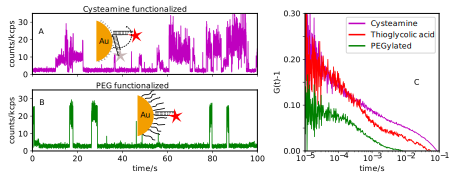
\includegraphics[width=\textwidth]{timetraceCysvsPeg}
	\caption{\textbf{Flexibility of the docking strand:} Time trace of transient binding on a gold nanorod with cysteamine (\ce{C2H7NS})(A) and mPEG7-SH (B) as passivating ligands.
	Notice the noisier intensity bursts in the case of cysteamine while the bursts for the PEGylated nanorod are much more stable.
	(C) Autocorrelation of intensity bursts for PEG (green), cysteamine (magenta) and thioglycol (red) functionalization.
	Autocorrelation values were obtained by averaging the individual autocorrelations from all bursts in each time trace. 
	Cysteamine and thioglycol have shorter chain lengths than PEG, and therefore allow more fluctuations of the distance between the nanorod and the imager dye (colored stars).}
  	\label{fig:timetraceCysvsPeg}
\end{figure}


The decay at shorter time scales (\SI{<1}{\ms}) present in all three cases is attributed to cis-trans conformational dynamics of Cy5.\cite{yeh2008tunable}
Cy5 can undergo cis-trans isomerization (Fig. S\ref{SIfig:AuNR-SS_bonding}). The trans form is planar and has stronger fluorescence, whereas the cis form has a distorted form with much lowered fluorescence.
The decay at longer time scales (\SI{\sim100}{\ms}) for cysteamine and thioglycol functionalization can be attributed to the interaction of the docking strand with the functionalized nanorod surface.
Although the movement happens at nanometer scales, it can be clearly observed because of the strong dependence of the enhancement on the position with respect to the tip of the nanorod.
As the docking strand wiggles, it can come close to the surface of the nanorod resulting in quenching or it can move away from the surface of the tip resulting in enhancement.
The persistence length of DNA\cite{manning2006the} is \SI{50}{\nm}, which suggests that the movement arises from the flexibility of the tether between the docking strand and the gold surface.
However, for PEG-functionalized nanorods, the slower fluctuations are missing. We attribute this to steric hindrance by PEG chains, which prevent interactions between the hybridized DNA and the gold surface. Although the PEG brush sterically hinders the DNA motion, the imager strands can still migrate into the brush and bind to the docking strand without compromising the transient binding.


%=======countrate vs duration==========
\paragraph{Binding time.}
The binding time of the imager to the docking strand depends on many factors: the number of base pairs involved in the binding, the salt concentration, the temperature.
For the current study, the number of base pairs involved in the binding was fixed to $10$ and all the measurements were performed at \SI{500}{\mM} \ce{NaCl} and at room temperature (\SI{298}{\kelvin}).
The length of the imager strand was chosen to be $10$ base pairs to get maximum fluorescence enhancement.
Khatua et al. obtained maximum fluorescence enhancement at a distance of \SIrange{3}{5}{\nm} from the tip of the gold nanorod for the low-quantum-yield dye Crystal Violet.\cite{khatua2014resonant}
Combining the length of DNA with that of the linkers between gold and DNA and between DNA and dye, we obtain a distance of \SI{\sim4}{\nm}, which should result in optimum enhancement.
The binding times of the imager observed from the time traces are plotted against the intensity of the bursts in the scatter plot of Figure \ref{fig:countrate_vs_duration}(A).
For low count rates we find more points with long dwell times, while at higher count rates, most of the bursts have short dwell times. 
The average burst duration clearly declines for count rates larger than \SI{\sim25}{kcps}.
We assign the reduction of burst duration for high count rates to bleaching of the dye. For low enough count rates, the burst duration will be limited by the binding time of the imager strand, rather than by the bleaching of the dye. We thus attribute the burst duration at low count rates (below \SI{\sim25}{kcps}) to the binding time of the imager.
Above \SI{\sim25}{kcps}, the dye bleaches before the imager strand unbinds from the docking strand, resulting in a shortened burst duration. We thus selected a maximum threshold of \SI{\sim25}{kcps} for estimating the binding kinetics. The histogram of binding times of intensity bursts with count rate less than \SI{\sim25}{kcps} is shown in Figure \ref{fig:countrate_vs_duration}(B), which appears to decay exponentially with a characteristic time of \SI{1.13}{\s}. The binding time of \SI{1.13}{\s} for 10-base-pair-binding at \SI{500}{\mM} \ce{NaCl} is similar to the value of \SI{5}{\s} obtained previously.\cite{jungmann2010singlemolecule}

\begin{figure}[ht]
	\centering
	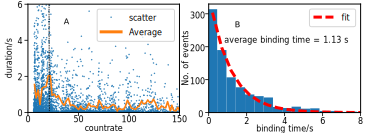
\includegraphics[width=\textwidth]{countrate_vs_duration_nophtns}
	\caption{\textbf{Binding time:} (A) Scatter plot of the burst duration versus count rate for intensity bursts in transient binding events. The data were obtained from $24$ nanorods with 1 to 5 docking sites on each of them. The vertical line indicates the count rate above which bleaching starts to govern burst duration.
	(B) Histogram of binding times of intensity bursts with count rates smaller than \SI{25}{ kcps}. The threshold was selected to exclude most bleaching events. From the exponential fit, we find an characteristic binding time of \SI{1.13}{\s}.}
  	\label{fig:countrate_vs_duration}
\end{figure}


%========Enhancement statistics=========
\paragraph{Enhancement distribution.}
Considering the strongly inhomogeneous near field of the nanoantenna, we expect a wide distribution of enhancement factors.
Figure \ref{fig:int_lt_distribution}(A) shows the distribution of burst intensities obtained for $24$ nanorods with 1 to 5 observable binding sites. The average count rate of all those bursts was \SI{53}{kcps}, corresponding to an average fluorescence enhancement factor of $\sim25$.
The possible positions of the dye at the tip of nanorod, assuming the tether to stand perpendicular to the surface, are shown in Figure \ref{fig:int_lt_distribution}.
The color map shows the optical intensity simulated by finite difference time domain (FDTD) in COMSOL. The lifetime histogram of enhanced fluorescence is shown in magenta (Figure \ref{fig:int_lt_distribution}(C)) while that of unenhanced fluorescence (in absence of intensity bursts) is shown in green.
The lifetime of unenhanced Cy5 is \SI{1.8}{\ns} while the lifetime histogram of enhanced bursts cannot be distinguished from the instrument response function.
\begin{figure}[ht]
	\centering
	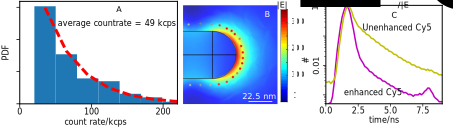
\includegraphics[width=\textwidth]{lifetime_scatplot}
	\caption{Enhancement statistics.(A) Histogram of count rates of intensity bursts of transient binding obtained from $24$ gold nanorods with 1 to 5 docking sites on each of them.
	The average count rate was \SI{53}{ kcps} with an enhancement factor of $\sim 25$.
	(B) Optical intensity map of the nanorod. The red stars indicate the positions the dye can occupy at the surface of the nanorod.
	The color bar is the normalized intensity.
	Both the enhancement factor and the number of possible binding sites are functions of the distance of the dye to the tip. The strongest enhancement corresponds to a small disk at the rod's tip, whereas the large areas on the rod sides correspond to much lower enhancements.
	(C) Lifetime histogram of all the intensity bursts found in the time trace of Figure \ref{fig:timetrace1vsmany}(a) shown in magenta. The lifetime histogram of the unenhanced fluorescence is shown in green.
	}
  	\label{fig:int_lt_distribution}
\end{figure}


As the docking strands are functionalized randomly on the nanorod without specificity to the tip, we expect to find enhancement factors corresponding to all possible positions of the dye at a fixed distance ( 4 nm) from the gold surface.
The maximum enhancement factor observed is 100, which is reasonable for a dye with a high quantum yield (\SI{30}{\percent}) and for an excitation enhancement of \SI{\sim300}{times} by the gold nanorod.
A previous study of the dye crystal violet showed an excitation enhancement of about hundred times. Because this dye has low quantum yield (\SI{1}{\percent}), a fluorescence enhancement of thousand-fold resulted from excitation enhancement and a 10-fold radiative enhancement. The radiative enhancement strongly depends on the quantum yield of the dye. Poorer quantum yields give rise to larger radiative enhancements. For Cy5 with a higher quantum yield, no significant radiative enhancement is expected, and the fluorescence enhancement is expected to stem mainly from excitation enhancement.
The most intense bursts come from close to the center of the tip while weak bursts originate from the sides.
The histogram of burst heights should thus be related to the distribution of light intensity at a distance of about \SI{4}{\nm} from the surface of the nanorod.


The lifetime histogram of enhanced fluorescence cannot be distinguished from the instrument response function. Therefore, the fluorescence rate (combining radiative and non-radiative rates) is enhanced by at least a factor of 10 (the lifetime of Cy5 away from the nanorod is \SI{1.8}{\ns}). However, with our current data, we cannot distinguish radiative from non-radiative contributions.
The previous study\cite{seelig2007nanoparticleinduced} shows that even at a distance of \SI{15}{\nm}, the lifetime is already reduced by a factor of 10.
As in the current study, the distance of the dye is just \SI{4}{\nm}, we expect a much shorter lifetime which requires a high-resolution TCSPC to be measurable.
% XXXrewrite this in a more neutral wayXXX As we don't expect much enhancement in the quantum yield of Cy5, quenching is probably a main contribution to the shortening of the lifetime.


\section{Conclusion}
We demonstrated the observation of many single molecules with equal enhancement factors on a single gold nanorod with a single binding site.
Different nanorods showed different enhancement factors because they presented different positions of the docking strand, in addition to different plasmon resonances.
Once a nanorod is identified with the desired enhancement factor, many single molecules can be studied with the same excitation and emission yields.
The effort to find the best enhancement factor can be reduced by specifically attaching the docking strand at the tip of the rod.
This transient binding method can be applied to different kinds of plasmonic nanostructures, where the position of the emitter can be controlled by proper DNA engineering.
Similarly, different biomolecules and quantum emitters can be studied by attaching them to the imager strand.

%=========================== SUPPORTING INFORMATION ==========================
\graphicspath{{chapters/c5_transient_binding/si-figures/}}
%============================ MAIN ==========================
\section{Supporting info}
\begin{figure}[ht]
  \centering
  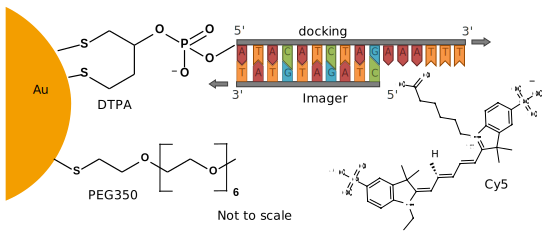
\includegraphics[width=0.8\textwidth]{AuNR-SS_bonding}
  \makeatletter
  \renewcommand{\fnum@figure}{\figurename~S\thefigure}
  \makeatother
  \caption{\textbf{Binding to gold surface} The chemical structures of different components in the transient binding scheme.
  The docking strand is attached to the nanorod through DTPA, which has two thiols attached to the gold atoms.
  The sequence of the docking and the imager strand are shown with their complementary binding.
  The imager strand is labeled with Cy5 at its 5' end.
  The rest of the nanorod surface is functionalized with PEG350, which has 9 monomers giving it a length of \SI{\sim3}{\nm}.}
  \label{SIfig:AuNR-SS_bonding}
\end{figure}

\begin{figure}[ht]
  \centering
  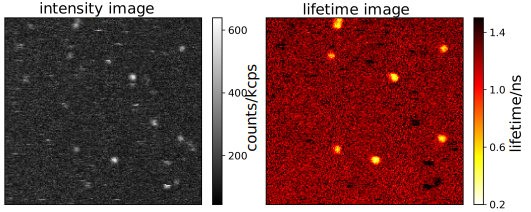
\includegraphics[width=0.8\textwidth]{trans_int_lt_img}
  \makeatletter
  \renewcommand{\fnum@figure}{\figurename~S\thefigure}
  \makeatother
  \caption{A \SI[product-units=power]{10x10}{\um} scanning image of the surface of the substrate with gold nanorod functionalized with docking strand and mPEG7-SH.
  The solution contains \SI{100}{\nM} imager strand in PBS pH 7.4 buffer with \SI{500}{\mM} \ce{NaCl}.
  The image on the left shows counts per millisecond while the image on the right shows the lifetime.
  The spots on the lifetime image correspond to the gold nanorods as they have a much shorter lifetime than the instrument response function.}
  \label{SIfig:trans_int_lt}
\end{figure}
% \subsection*{Replenish and recyacle}
\begin{figure}[ht]
  \centering
  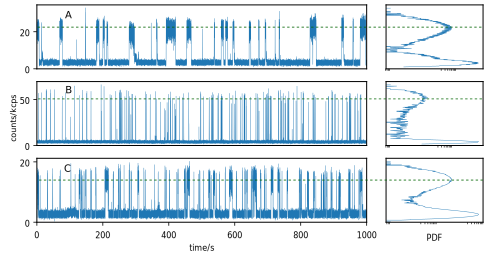
\includegraphics[width=\textwidth]{bleaching_free_longtrace}
  \makeatletter
  \renewcommand{\fnum@figure}{\figurename~S\thefigure}
  \makeatother
  \caption{\textbf{Many single molecules bind to the same binding spot on the same nanorod.} Time traces of three different nanorods, each of them with a single binding site, but with different enhancement factors.
  The histogram of intensities for each time trace is shown on the right and the two peaks indicate the presence of only one observable docking strand.
  Notice the different binding kinetics of trace A and trace C although they have similar enhancement factors.}
  \label{SIfig:bleaching_free_longtrace}
\end{figure}

\begin{figure}[ht]
  \centering
  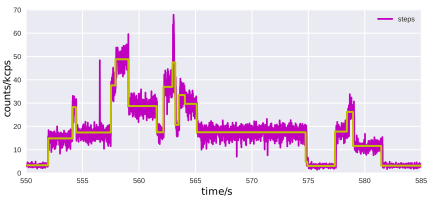
\includegraphics[width=\textwidth]{step_timetrace}
  \makeatletter
  \renewcommand{\fnum@figure}{\figurename~S\thefigure}
  \makeatother
  \caption{\textbf{Multi-step transient binding:}Time trace on a functionalized gold nanorod with multiple transient binding events appearing on top of each other.
  The association and dissociation of each imager strand can be distinguished from the step height and the time of appearance. }
  \label{SIfig: step_transbind}
\end{figure}

% \subsection*{Transient binding on substrate}
\begin{figure}[ht]
  \centering
  \includegraphics[width=\textwidth]{timetrace_only_Cy5}
  \makeatletter
  \renewcommand{\fnum@figure}{\figurename~S\thefigure}
  \makeatother
  \caption{\textbf{Transient binding without nanorod:} (A) Schematic of the transient binding.
  The docking strand was immobilized on the surface through neutravidin and biotin bonding.
  The solution contained \SI{100}{\nM} imager-Cy5 in PBS pH 7.4 buffer.
  Scanning image  in the absense (B) and presence (C) of docking strand on the surface showing the specificity of binding of the imager to the docking strand.
  (D) Time trace of transient binding on a single neutravidin-docking site at \SI{\sim 0.1}{\kW\per\cm\squared} power density, 10 times higher than the laser power used for measurement on the nanorod. The burst heights are \SI{\sim 20}{ kcps} corresponding to single imager-Cy5.
  To compare with the bursts from nanorods and calculate the enhancement factor, the count rate can be divided by 10 to match the laser power on the nanorod as the intensity varies linearly at such low powers.
  A count rate of \SI{2}{ kcps} for unenhanced Cy5 has been used in the main text. 
  }
  \label{SIfig:timetrace_only_Cy5}
\end{figure}
% \subsection*{Dissociation of docking strand}
\begin{figure}[ht]
  \centering
  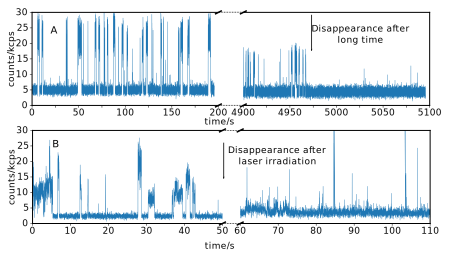
\includegraphics[width=\textwidth]{dissociation_transbind}
  \makeatletter
  \renewcommand{\fnum@figure}{\figurename~S\thefigure}
  \makeatother
  \caption{\textbf{Dissociation of docking strand.}
  (A) The time trace on the top is recorded on a gold nanorod until no docking events any more are observed.
  The transient binding events never reappeared, even after re-flushing with imager strand and realigning the laser focus.
  (B) The transient binding trace on a gold nanrod before and after irradiation with high laser power (\SI[per-mode=repeated-symbol]{1000}{\watt\per\cm\squared}, \SI{40}{\MHz}).
  }
  \label{SIfig:dissociation_transbind}
\end{figure}
% \references{chapters/c5_transient_binding/transient_binding}
\chapter{Redox activity of Single-azurin at diffferent electrochemical potential}
% !TeX root = ./azurin.tex
\graphicspath{{./chapters/c4_azurin_sm/main/}}
% \externaldocument{./chapters/c4_azurin_sm/si_azurin} 
%%%%%%%%%%%%%%%%%%%%%%%%%%%%%%%%%%%%%%%%%%%%%%%%%%%%%%%%%%%%%%%%%%
%%%%%%% Start the main part of the manuscript here.%%%%%%%%%%%%%%
%%%%%%%%%%%%%%%%%%%%%%%%%%%%%%%%%%%%%%%%%%%%%%%%%%%%%%%%%%%%%%%%%%
\section{Introduction}
Introduction here.
%%%%%%%%%%%%%%----------EXPERIMENTAL SECTION----------%%%%%%%%%%%%%%%%%%%%
\section{Experimental Section}
\subsection{Protein synthesis}
Azurin (wild type) from Pseudomonas aeruginosa was expressed in E. Coli and purified as described before \citep{kamp1990purification}. BL21 E.coli was transformed with PGK22 plasmid that has gene for azurin expression. The cells were cultured in luria broth (LB) medium. Then the cells were harvested and resuspended in 20 \% (w/v) sucrose solution in Tris pH 8 buffer containing $1~$mM EDTA.The solution was centrifuged at $8000~$rpm and the supernatant was collected. Copper sulfate was added to the solution for insertion into the active site of azurin. The unwanted proteins were precipitated by addition of acetic acid until pH 4. Again the turbid solution was centrifuged to separate azurin that remained in the supernatant. The azurin solution was loaded on a CM Sepharose fast flow column and elution was performed in an Akta purifier (GE Healthcare) with a pH gradient from $4$ to $6.9$ in $50~$mM ammonium acetate. Fractions containing azurin collected and reduced with sodium dithionite. At this moment the solution had both zinc and copper azurin. The azurins were purified in a DEAE sepharose column by a salt gradient of 0 to $50~$mM NaCl in Tris pH8 buffer. Fractions containing copper azurin and zinc azurin collected and concentrated separately. The purity of the samples were checked by sodium dodecyl sulphate (SDS)-polyacrylamide gel electrophoresis (PAGE) and UV/Vis spectroscopy (Cary 50 spectrophotometer, Varian Inc., Agilent Technologies, USA). The azurins appeared on SDS gel page at \~14 kDa. Both zinc and copper azurin showed a characteristic peak at ${\sim}290~$nm while Cu azurin showed an additional broad absorption peak at $620~$nm as can be seen in Figure-S\ref{SIfig: switching} when oxidized. The ratio $O.D_{628nm}/O.D_{280nm}$ for Cu azurin was 0.56 which indicated that all the azurin molecules had a Cu atom. The concentrated protein was stored at $-80^0 C$ until further use.
\subsection{Fluorescent labeling}
The labeling protocol was based on the previous work \cite{nicolardi2012topdown}. ATTO 655 NHS-ester was bought from ATTO-TEC GmbH. The buffer containing azurin was replaced with HEPES pH 8.3 and all the amine containing impurities were removed. ATTO655 was chosen to label the protein because of its stability and light insensitivity in the interested potential range. A mixture of 200~$\mu$M azurin and ATTO 655 NHS-ester (ration 1:1) was incubated for 45~min. The NHS-ester group reacts to one of the amine group on the protein. The unreacted dyes were removed by a HiTrap desalting column. The labeled protein was concentrated in Tris pH 8.5 buffer by centrifuging in a 3~kDa Amicon ultra filter. The labeled protein further purified by an ion exchange chromatography in a 1 mL MonoQ column (GE Health). The different peaks obtained (see figure S\ref{SIfig: peak_sep}) corresponds to the different number and position of the dye on azurin. The peak-III corresponds to the protein labeled at Lysine122 position \cite{nicolardi2012topdown}. For this position of the dye, the protein construct shows high fluorescence switching (90\%) ratio between oxidized and reduced condition as can be seen in Figure S\ref{SIfig: peak_sep}. This fraction was choosen for our single-molecule experiment as the two states can be observed easily. The same protocol was used for Zn azurin labeling and similar peak separation observed. The fluorescent labeled protein was then reacted with biotin-peg-NHS (MW 3400) in PBS pH 7.4 buffer with a ratio 1:5 to make sure each protein has at least one biotin. The free biotin was then removed by centrifuging in a 3kDa Amicon ultra filter. The biotin on the protein will be used for immobilization on glass surface.
\subsection{Functionalization of cover slips}
The functionalization of glass surface was followed from a previous work with a little modification.\cite{gupta2012involvement} Glass coverslips (Menzel-Glaser, $22~mm \times 40~mm$, no. 1 thickness) were used for immobilization.The cover slips were sonicated in water (15 min) and acetone(15 min). Then they were rinsed in Milli-Q water several timesand incubated in a H2O/NH4OH/H2O2(5:1:1) bath at \SI{70}{\celsius} for burning all the organic impurity on the surface. The coverslips were rinsed several times with water and ethanol and finally stored in ethanol. Before functionalization, the slides were flamed. Then they were treated for 30 min with a 1\% solution of [3-(2-aminoethyl)aminopropyl]trimethoxysilane in methanol containing 5\% glacial acetic acid. This results in the binding of the active hydroxyl groups. The silane is not yet covalently bound. This is obtained by baking the cover slips in an oven at \SI{65}{\celsius} for 3 hours. After this treatment, the cover slips were sonicated for 10 minutes and washed with methanol. Dried with clean nitrogen, they were left in a desiccator overnight. The next day they were treated with a mixture of 5~mg/mL methoxy-peg-N-hydroxysuccinimide (MW~2000, Laysan Bio) and 0.05~mg/mL
biotin-peg-N-hydroxysuccinimide (MW 3400, Laysan Bio) in 50 mM phosphate buffered saline (PBS) with pH 7.4. This creates a surface containing biotin and methoxy end groups. The PEG surface prevents nonspecific adsorption of the protein. The slides were dried with gentle flow of nitrogen and stored in a desiccator until further use.
\subsection{Protein immobilization}
The above biotin functionalized glass slide was incubated with $20~$mM PBS pH 7.4 buffer for $5~$min. $100~$nM of Neutravidin (Thermo Scientific) was incubated for another $15~$min and then washed to remove unbound Neutravidin. $100~$pM of the labeled protein was then incubated for $1~$min to get isolated proteins (20 per \SI{100}{\micro\meter} area) on the functionalized glass surface. The unbound proteins were then removed by replacing with a fresh PBS buffer.
\subsection{Electrochemical-potential control}
Once the unbound proteins are removed, a new mixture containing $0.1~$mM sodium ascorbate ($[C_6H_7O_6]^-Na^+$) and $0.2~$mM potassium ferricyanide ($[Fe(CN)_6]^{3-}$) in $4~$mL PBS pH 7.4 was added at the sample holder which were our initial oxidant and reductant. Electrochemical potential of the solution is obtained from the ratio of oxidant and reductant. The solution potential was controlled with the same electrochemical set up as previously described\cite{zhang2017gold} with little modification. A potentiostat (Model 800B Series Electrochemical Detector, CH Instruments) was used to apply electric potential. A platinum rectangular grid (the total length/ width of the grid is around $2.5~$cm) was used as working electrode and pressed onto the sample slide with the help of a small glass slide. Not only is the pressure evenly applied on the grid, but also small confined volumes are formed where the sample slide and glass slide form the `floor' and `roof' and the platinum grid forms the `walls'. A part of the platinum grid was exposed to the solution. These confined volumes are in the order of nanoliters, which makes switching of elctrochemical potential of solution possible in a matter of minutes.
\subsection{Confocal Microscope}
Single-molecule measurements were carried out in a home built confocal microscope. The setup was equipped with $635$ nm pulsed diode laser (Power Technology, Little Rock, AR, USA) controlled by PDL 828 "Sepia II" (PicoQuant) at $40$ MHz repetition rate. the laser beam was passed through a narrow-band cleanup filter (Semrock LD01-640/8-25) and coupled a single-mode optical fiber to obtain a Gaussian beam profile. The output beam was collimated and reflected by a polychroic mirror (z488/633rpc) onto the back aperture of an oil immersion objective (NA=1.4, Olympus UPLSApo 100x). The sample holder with the glass slide and electrodes were mounted on a scanning stage (Physik Instrumente P-517.3CD) controlled by nanopositioning system (Physik Instrumente E-710.3CD). The epifluorescence light was collected back through the same objective and focussed on a \SI{50}{\micro\metre} pinhole for spatial filtering, then passed through an emission filter (z488/635m "dual"-band emission filter, Chroma). The fluorescence beam was re-collimated and focussed on single-photon avalanche photo diodes (SPCM AQRH-15, Perkin Elmer Inc., USA). The signal from the photo diode was recorded by a PicoHarp 300 (PicoQuant GmBH, Berlin, Germany) in time-tagged-time-resolved mode.
\subsection{Data recording}
A $20$ by $20$ \SI{}{\micro\metre}$^2$ area of the sample surface functionalized with sparsely distributed ATTO655-labeled Azurin was scanned with $50$~nm per pixel and with a dwell time of $1$~ms per pixel. A typical fluorescence intensity image can be seen in Scheme-\ref{sch:setup}. A constant potential of $200$~mV (oxidizing) was applied by the electrochemical analyzer and an image of the same area taken after $2$~min. Typically within one minute, the solution potential of the mixture of $0.1$~mM ascorbate and $0.2$~mM ferricyanide reaches the applied potential. Another image of the same area recorded at $0$~mV (reducing). The two images were compared to identify the molecules that switch on-off at the two potentials (Scheme-\ref{sch:setup} (9 \& 10)). The coordinates of the switching molecules were registered and an automatic recording was started. For each molecule, time traces were recorded for $30$~s at different potentials between $-100$~mV and $100$~mV. For observing dynamic of a single-molecule over longer period, time traces were recorded until the dye on it bleached or became dead. The Zn-azurin-ATTO655 was used used as a control which doesn't show switching it's intensity at the above two potentials and time traces were recorded at the same potentials as Cu-azurin.
\subsection{Data analysis}
All the measurements resulted a huge amount data (more than $1000$ time traces). Each time trace contains absolute arrival times of photons as well as arrival time with respect to excitation laser pulse. This enabled us to extract maximum information from the traces. To minimize human error and attain efficiency, codes were written (in python, matlab) to analyze all the traces exactly the same way. The code and data ca be found in the given link (will be provided during submission). Mainly three analysis were made on each trace. (i) Change points in the time traces were obtained using the changepoint algorithm\cite{watkins2005detection} kindly provided by Prof. Haw Yang (Princeton University, USA). This method is binning free and doesn't require any prior knowledge of the underline kinetics. It determines the location of intensity changes based on the photon arrival times and the algorithm is recursively applied through the whole trace to find all the changes. Bayesian information criterion is used to find the number of states. Two states were predicted from long time traces and many molecules (2500 changepoints each) with more than 90\% accuracy which was expected from FRET quenching mechanism and total signal that we have. For the rest of the traces, we set the number of states to be two in order to minimize the computation time. An example of change points and it's overlap with the real time trace can be seen in Figure-\ref{fig:timetrace}. (ii) Autocorrelation of the time traces were performed by using SymPhoTime(PicoQuant) software. (iii) Further analysis of changepoint outputs and autocorrelation outputs were performed in Python. The details of the code including all the fitting functions can be found in the online repositories (will be provided during submission).
%Scheme
\begin{figure}
	\centering
	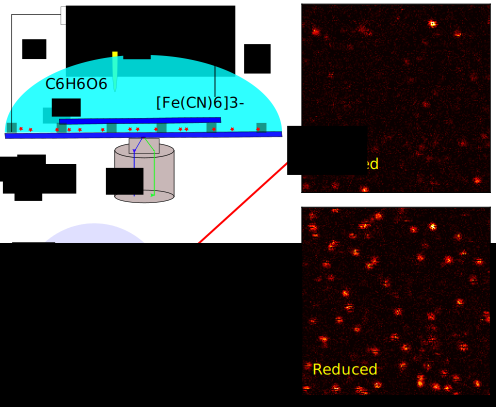
\includegraphics[width=\textwidth]{Scheme_1_setup.eps}
	\caption{The schematic picture of the confocal and electrochemical setup. \textbf{(1)} Objective through which light is irradiated on and collected from the sample. \textbf{(2)} The functionalized sample slide with on top the platinum grid and another small glass slide to press the grid on the sample slide, resulting in small confined volumes in the order of nanoliters. \textbf{(3)} The electron mediator solution consisting of $200~$\uM~ferricyanide, $100~$\uM~ascorbate in PBS (PH 7.4) buffer with a total volume of 4 mL. \textbf{(4)} The working electrode (Platinum wire) that is in contact with the platinum grid. \textbf{(5)} The saturated calomel reference electrode. \textbf{(6)} The Platinum wire (not touching the grid) as counter electrode. \textbf{(7)} The potentiostat (Model 800B Series Electrochemical Detector, CH Instruments) to which the electrodes are connected. \textbf{(8)} Top view of the sample slide and two images are showing the labeled Cu-Azurin reduced (brighter) and oxidized (dimmer).}
  	\label{sch:setup}
\end{figure}
%%%%%%---------------------RESULTS and DISCUSSION-----------------------%%%%%%%%%
\section{Results and discussion\label{sec:results}}
\subsection{Time traces at different potentials}
Active Cu-azurin molecules were identified from their fluorescence intensity images at the oxidizing ($200~$mV) and reducing conditions($0~$mV). In reducing conditions, the image contains more brighter spots corresponding to Cu(I)-azurin-ATTO655 and more than $90~$\% of the molecules turned off in oxidizing conditions (Scheme-\ref{sch:setup}(9)). The azurins on each sample slide showed active switching during the course of our experiment (upto two days) without any noticeable degradation. A set of active azurins were marked for recording and time traces at different potentials (between $100~$mV and $-100~$mV) were measured on the \texttt{same molecules} for $30~$s. Many of the labeled-protein bleached within recording at few potentials, but more than $50~$\% of the labeled-azurin survived at least five measurements ($150~$s) at different potentials. Longer measurements were possible due to the scavenging of oxygen in the solution. Before the time trace recording, the solution was exposed to negative potential for at least $1~$hours. Ascorbate is known to  scavenge oxygen\cite{dave1997effectiveness} and get oxidized. The oxidized ascorbate is reduced by the electrode and was again available to scavenge other oxygen molecules. In addition to the absence of oxygen, the ROXS mechanism was also in play. The reduction and oxidation of Cu-azurin made the dye switch on and off, hence the fluorescent dye spent less time on the bright state where it is more prone to bleach. This made possible the measurement of some traces more than $1000~$s long.\\
%---time trace
\begin{figure}
	\centering
	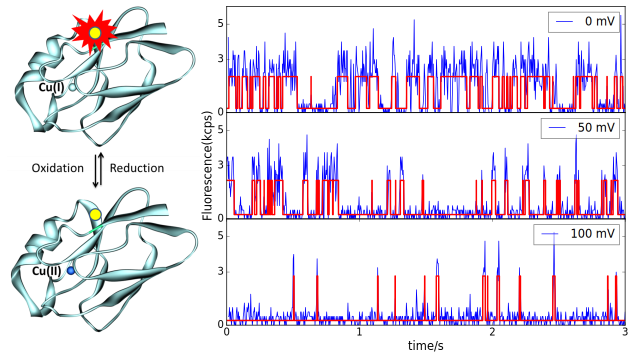
\includegraphics[]{Figure_1_timetrace_CuAzu.eps}
	\caption{Time traces of Cu-Azurin labeled with ATTO655 at different potentials. The structure of the protein with properly positioned dye can be seen in the schematic picture in the left. In Cu(II) state (shown in bluish atom in the protein structure), the dye is non fluorescent because of FRET and in Cu(I) state (shown in gray atom), the dye is fluorescent. Notice the amount of time the protein spends on bright and dark state at different potentials. At lower potentials (e.g 0 mV) the protein is brighter most of the time because of the higher concentration of reductant.}
	\label{fig:timetrace}
\end{figure}
Figure-\ref{fig:timetrace} shows time traces of a single Cu-azurin-ATTO655 at three different potentials. Clearly the intensity changes from bright to dark and vise versa over the time which is also schematically shown in the left of Figure-\ref{fig:timetrace} with the protein structure. The dark state is due to the FRET from the dye to the Cu(II) absorption center\cite{kuznetsova2006a}. Bulk measurements of the fluorescence intensity at completely oxidizing and completely reducing condition shows $90~$\% switching ratio (Figure-S\ref{SIfig: switching}) for the lysine-122\cite{nicolardi2012topdown} labeled Cu-azurin-ATTO655. Also single-molecule measurement (Figure-S\ref{SIfig: lifetime}) at a higher laser power (\SI{0.7}{\micro\watt}) shows more than $90~$\% switching which is consistent with the bulk measurements. The intensity of Cu(II)-state is lower than Cu(I)-stae, but higher than the background (bleached state). Also the Cu(II)-state has a shorter lifetime($0.3~ns$ than Cu(I)-state ($1.9~ns$), but longer than the instrument response function ($0.1~ns$). Both intensity and life time information reassure us that the dim-state we looking at is FRET quenched. Other blinking mechanism appears at lower potentials which will be discussed later. The high FRET efficiency is due to the small distance of the dye to the absorption center. This clear distinction between the on and off state was very important for our low laser power and lower signal measurement. At higher potential ($100~$mV), the protein spends most of the time in dark state and as the potential is lowered, the molecule spends more and more time on the bright state. As we lower the potential, the concentration of the reductant increases keeping the protein in Cu(I)-state for longer time. A control study with Zn-azurin-ATTO655 (Figure-S\ref{SIfig:tracecomparision} and Figure-S\ref{SIfig:fcscomparision}) shows that the dye itself blinks below $40~$mV due to photo-excited electron transfer. Zinc does not absorb light in the red and does not switch it's oxidation state. To leave out the complication in the analysis procedure, only potentials above $40~$mV were considered for Cu-azurin-ATTO655 study.\\
%Midpoint histogram
\subsection{Midpoint potential of single-azurins}
\begin{figure}
	\centering
	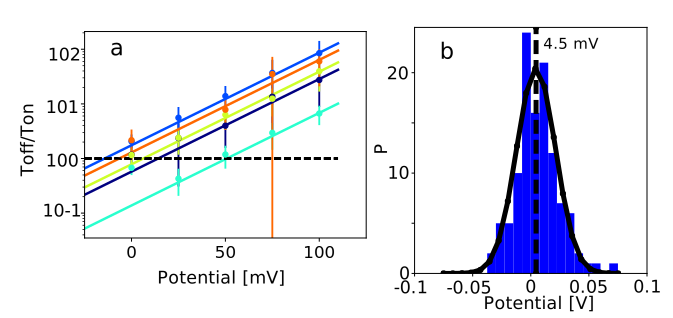
\includegraphics[]{Figure_2_midpoint.eps}
	\caption{Ratio between on and off time as a function of applied potential for the same single-molecule. Different color represents different single-molecules. And the line connecting the data points is the Nernst fit for all the data points above 25 mV. The plot in the right is the histogram of midpoint potentials for $132$ molecules with a Gaussian fit with a center value of 4.5 mV with respect to calomel electrode.}
	\label{fig:midpoint}
\end{figure}
Figure-\ref{fig:midpoint}a shows the ratio between average off-time and average on-time plotted against the applied potential. The linear relationship of the log of the ratio with the potential can be modeled with the Nernst equation: 
\begin{equation}
	E = E_0 + \frac{k_BT}{n e}\ln\left(\frac{\me{t}_{on}}{\me{t}_{off}}\right)\,
	\label{eq:nernst}
\end{equation}
where $E$ is the applied potential, $E_0$ the mid-point potential, $k_B$ the Boltzmann constant, $T$ the absolute ambient temperature, $n$ the number of electrons involved in the reaction, $e$ the electron charge and $\me{t}_{on}$, $\me{t}_{off}$ the mean on and off times. The number of electrons involved in the electron transfer was set to $1$. The value of $n$ was also found to be one from the ratio plot when the slope in the Nernst equation kept as free parameter (see Figure-S\ref{SIfig:potential_slope}). Each color represents a single-azurin and the solid line connecting the points is the Nernst-fit. Labeled proteins surviving at least three potentials above $40~$mV were used for the fit. The potential at which the off-on ratio is $1$ called midpoint potential which means the probability of finding the protein in Cu(I) and Cu(II) state are the same. The distribution of mid-point potentials(Figure-\ref{fig:midpoint}b) from 132 molecules can be fitted by a Gaussian with a center value of $\left<E_0^{SM}\right>=4.5 \pm 1.2~$ mV and a full width half maximum (fwhm) of $\sigma^{SM}=36 \pm 3~$ mV. The midpoint potential values are similar to previously reported values of $6\pm0.6~$mV with fwhm=$150~$mV where each $E_0$ was calculated from about $1000$ molecules.\cite{davis2006monitoring} Another work reported $E_0 = 16~mV$ with low surface coverage (100s of azurins) with a fwhm of $70~$mV.\cite{salverda2010fluorescent} Recently for truly single-azurin, $E_0=12\pm3$ was reported with fwhm of $92~$mV.\cite{akkilic2014chemically-induced}\\
A small width of distribution ($36~$mV) for single-azurin potentials in this work is obtained probably because of the way the proteins are functionalized to the surface. The azurin is attached to a peg-chain of length ${\sim}20~$nm. The peg-chain is attached to the surface through neutravidin. Such functionalization minimizes the interaction of the protein to the surface. In all the previous experiment, the azurin was either non-specifically attached to the surface or attached through a very small linker (<$1~$nm).
%====================Many single-molecule on-off histogram and their rates=================
\subsection{Intermediate detection from on-off histogram}
\begin{figure}
	\centering
	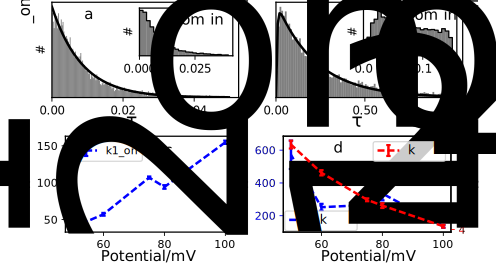
\includegraphics[width=\textwidth]{many_sm_hist.eps}
	\caption{\textbf{Electron transfer rates} The histogram of on-times (a) and of off-times (b) of all the single-Cu-Azurin-ATTO655 at $100~$mV with their zoomed in part in the inset. Notice the single exponential decay of on-times and bi-exponential (with rise time) for the off-times. This indicates that  reduction of Cu-Azurin occurs through an intermediate step while for oxidation the intermidiate state is not observable. The solid line is the corresponding fit to the distribution. (c) The rate constant for oxidation as a function of potential. (d) The rate for reduction as a function of redox potential, blue points correspond to the faster rate constant and the red represents the slow rate constant.}
	\label{fig:many_sm_hist}
\end{figure}
The on and off times of all the molecules at a certain potential were put together to see over all distribution. Figure-\ref{fig:many_sm_hist}(a) shows the histogram of on times at $100~$mV and the solid line is a fit with a single exponential with a time constant ($k_{on}$) of $155~s^{-1}$. The on-time represents the time the protein takes to get oxidized which can be shown as following:
\begin{align}
	\ch{!(bright)(Cu(I)Azurin) + oxd <=>[ $k_1$ ][ $k_{-1}$ ] !(dark)(Cu(II)Azurin) + red }
	\label{eq:oxidation}
\end{align}
In contrast, the distribution of off-times shows non-exponential distribution with a rise time Figure-\ref{fig:many_sm_hist}(a). In the inset, the zoomed in part shows clearly that the probability of finding the protein with very short off-time is smaller. This distribution can be explained by Michaelis-Menten mechanism:
\begin{align}
	\ch{!(dark)(Cu(II)Azurin) + red <=>[ $k_1$ ][ $k_{-1}$ ] !(dark)(Cu(II)Azurin*red) -> [ k2 ] !(bright)(Cu(I)Azurin) + oxd}
	\label{eq:reduction}
\end{align}
where $k_1$ is the pseudo-first order rate constant which depends on the concentration of reductant and $k_2$ is the zero order rate constant which should be independent of the concentration of the substrate. By assuming $k_{-1}=0$, the probability of off time can be given as:\cite{lu1998single-molecule}
\begin{equation}
	P_{off}(t) = \frac{k_1k_2}{k_2-k_1} [exp(-k_1t)-exp(-k_2t)]
	\label{eq:2exp_risetime}
\end{equation}
At $100~$mV, $k_1$ for the reduction is $4.1~s^{-1}$ while $k_2$ is $135~s^{-1}$. The rates were determined at different applied potential. A linear relationship is observed between the rate of oxidation and the solution potential (Figure-\ref{fig:many_sm_hist}(c)). This is in agreement with the first-order kinetic dependent on the concentration of substrate as the concentration of electron mediators vary exponentially with the solution potential. From the slope of the line, a rate constant of $9.4\times10^6~M^{-1}s^{-1}$ for the oxidation is obtained. Similar linear relationship was observed for the $k_1$ of the raduction process as expected with a rate constant of $1.7\times10^5M^{-1}s^{-1}$.\\
The rate constant ($k_2$) for the second step in the reduction process has a weak dependence on the solution reduction potential(Figure-\ref{fig:many_sm_hist}(d, blue)). The value is around ${\sim}250s^{-1}$ which is more than an order of magnitude smaller than the rate of intermediate formation.\\
%==================Dynamics: Single-azurin over time===================
\subsection{Dynamics in ET rate}
After looking at many single-azurins, we investigated a single-azurin for long time. Figure-\ref{fig:long_azurin_trace} shows the statistics of a single-azurin at $100~mV$ that survives for ${\sim}1250~s$. The distribution of on and off times are similar to that of many single-azurin distributions.
%long_azurin_trace
\begin{figure}
	\centering
	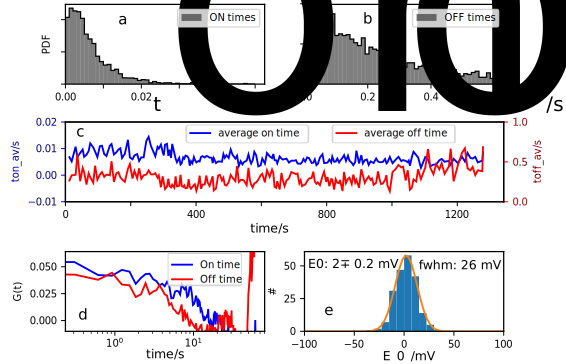
\includegraphics[width=\textwidth]{long_azurin_trace.eps}
	\caption{The histogram of on-times(a) and of off-times(b) of Cu-Azurin-ATTO655 showing rise time similar to many single-azurin distributions. (b) the trace of average on-times (blue) and average off-times (red). The average was calculated every $20$ corresponding on or off times. The respective y-scales have the same color as the data points. (d) Autocorrelation of the traces in (c) and the color is matched to the color in the trace. (d) distribution of $E_0$ calculated from each average on and off time from the traces in (c)}
	\label{fig:long_azurin_trace}
\end{figure}

The time trace was divided into small parts and average was calculated over every $20$ on or off times. Figure-\ref{fig:long_azurin_trace}~(c) average on-times (blue) and average off-times (red) as a function of time. To our surprise, the fluctuations are not simply statistical noise rather seems correlated. The autocorrelations of the average traces show clear decay (Figure-\ref{fig:long_azurin_trace}(d)) with decay times around $10s$ of seconds. This means that the rate at which the azurin change between Cu(II) and Cu(I) state varies over time. Sometimes the frequency of the state-change is low and sometimes it is high. Such behaviors has been observed previously for other enzymes ($\beta$-galactosidase, flavoenzymes).\cite{lu1998single-molecule,kou2005single-molecule,english2006ever-fluctuating} which can be termed as breathing in enzymes. A short on-time is followed be a short on-time and a longer on-time is followed by a longer on-time with the memory lasting over a characteristic time scale of $10s$ of seconds. According to the previous report, the breathing is a result of slow fluctuations in the structure over time. Azurin is a very small protein ($14$kDa) and the observation of such variation in ET shows that the ET is very sensitive to the changes in the structure.\\

Also mid-point potentials were calculated from each average on and average off times using Nernst equation(\ref{eq:nernst}). As both on and off times changes over time, mid-point potential too changes over time. The distribution of $E_0$ shows a center value of $2\pm0.2~$mV with a fwhm of $26~$mV. This distribution of midpoint potential of a single-azurin over a long time is similar to the value of $36~$mV obtained for many single-azurins.
%=================CONCLUSION==================
\section{Conclusion}
The results presented here shows how to controllably switch the solution potential and determine the switching ratio of redox active azurin. By introducing non-interacting surface and long linker, very narrow distribution in the midpoint potential obtained. The distribution over many single-azurin was found to be very close to the distribution of a single-azurin over long time. The rate of intermediate formation for the reduction process has been observed conferring to Michaelis-Menten mechanism. The intermediate formation for the oxidation was too fast to be detected with our signal to noise ratio. In principle similar measurement at higher laser power and for many molecule should enable the detection of the intermediate if their is any. For the first time, correlated dynamics observed in the ET of very small azurin whose molecular mechanism still need to be deciphered.

% \references{chapters/c4_azurin_sm/azurin}

%========bibliography===========
% \newpage
\references{bibliography}
%=========Apendix===============
\appendix

%% Turn off thumb indices for unnumbered chapters.
\thumbfalse
\end{document}